\documentclass[eng,printmode,openany]{mgr}
\usepackage[utf8]{inputenc}
\usepackage{polski}
\usepackage[polish]{babel}
\usepackage{graphicx}
\usepackage{subfigure}

\usepackage{psfrag}
\usepackage{amsmath}
\usepackage{amsfonts}

\usepackage{supertabular}
\usepackage{array}
\usepackage{tabularx}
\usepackage{hhline}
\usepackage{showlabels}
\usepackage{float}
\usepackage[square,sort,comma,numbers]{natbib}
\usepackage{multirow}

\usepackage{url}
\def\UrlBreaks{\do\/\do-}
\usepackage{breakurl}


\newcommand{\R}{I\!\!R}
\newtheorem{theorem}{Twierdzenie}[section]

\usepackage{listings}
\usepackage{xcolor}
\colorlet{punct}{red!60!black}
\definecolor{background}{HTML}{EEEEEE}
\definecolor{delim}{RGB}{20,105,176}
\colorlet{numb}{magenta!60!black}

\renewcommand\lstlistingname{Listing}
\renewcommand\lstlistlistingname{Listingi}

\lstset{
	basicstyle=\small,
	breaklines=true
}

\lstdefinelanguage{json}{
	string=[s]{"}{"},
	stringstyle=\color{blue},
	comment=[l]{:},
	commentstyle=\color{black},
}
% frontpage
\title{Aplikacja webowa wspomagająca zarządzanie flotą samochodów}
\engtitle{A web application supporting cars fleet management}
\author{Jan Pajdak}
\supervisor{dr inż. Jarosław Mierzwa, K-9}
\guardian{dr hab. inż. Olgierd Unold Prof. nadzw. PWr, K-9}
\field{Informatyka (INF)}
\specialisation{Inżynieria systemów informatycznych (INS)}

\begin{document}
	%\bibliographystyle{plabbrv}
	\bibliographystyle{plainnat} 
	
	\maketitle
	%\dedication{6cm}{dedykacja \texttt{$\backslash$dedication}}
	
	\tableofcontents 
	
	%----------------------------------------------------------------------------------------
	%	SECTION 0
	%----------------------------------------------------------------------------------------
	
	%----------------------------------------------------------------------------------------
	%	SECTION 1
	%----------------------------------------------------------------------------------------
	% cel, zakres pracy
	\chapter{Wprowadzenie}
	\section{Wstęp}
	Celem niniejszej pracy dyplomowej jest opracowanie projektu, implementacja oraz wdrożenie systemu umożliwiającego zarządzanie flotą samochodów. Pierwszym etapem projektu jest zebrane wymagań funkcjonalnych i niefunkcjonalnych oraz określenie zakresu pracy. Drugi etap projektu to wybór technologii i projekt architektury. Ostatnim celem jest implementacja systemu.
	
	Temat projektu został wybrany ze względu na chęć wykorzystania wiedzy z dziedziny motoryzacji w celu stworzenia aplikacji ułatwiającej zarządzanie pojazdami. Z uwagi na rosnącą popularność rozwiązań związanych z wypożyczaniem samochodów celem projektu jest system, który można opisać jako wewnątrzfirmową wypożyczalnie umożliwiająca jak największe wykorzystanie dostępnej floty pojazdów przez pracowników, którzy nie mają potrzeby posiadania firmowego samochodu na wyłączność. 
	
	\section{Cel i zakres pracy}
	Celem projektu jest stworzenie aplikacji umożliwiającej zarządzanie flotą samochodów. Aplikacja jest skierowana do firm które nie mają potrzeby lub wystarczających środków by zapewnić pracownikom samochody na wyłączność. Przykładowym przypadkiem użycia systemu może być jednorazowa potrzeba odwiedzenia klienta lub wyjazd na szkolenie. Typowe rozwiązania dla firm obecne na rynku skierowane są do firm świadczących usługi spedycyjne — aplikacje posiadają warstwę śledzenia ładunków oraz tworzenia zadań przewozowych dla kierowców; programy służące do obsługi komercyjnych wypożyczalni pomijają proces autoryzacji rezerwacji — zwykle sprawdzana jest zdolność wypożyczającego do zapłaty.
	
	Projekt utworzony w ramach tej pracy łączy mechanikę z komercyjnych wypożyczalni z dodatkową warstwą biznesową pozwalającą kontrolować sposób używania pojazdów.
	
	Zakres pracy obejmuje utworzenie systemu spełniającego wymagania postawione w rozdziale 3.
	
	\section{Układ pracy}
	W rozdziale pierwszym zawarto wstęp oraz krótki opis celu projektu. Drugi rozdział porównuje istniejące rozwiązania do aplikacji będącej celem projektu. Rozdział trzeci zawiera wymagania funkcjonalne oraz niefunkcjonalne. W kolejnym, czwartym rozdziale znajduje się opis wybranych technologii oraz narzędzi, wraz z uzasadnieniem. Rozdział piąty skupia się na opisie technicznym projektu oraz jego implementacji. Szósty rozdział zawiera opis sposobu testowania systemu. Ostatni, siódmy rozdział zawiera podsumowanie projektu.
	
	%----------------------------------------------------------------------------------------
	%	SECTION 2
	%----------------------------------------------------------------------------------------
	\newpage
	\chapter{Istniejące rozwiązania}
	Jednymi z popularniejszych rozwiązań obecnych na rynku są \textit{Fleetly} oraz \textit{Vinity Fleet Manager}. Sposób działania \textit{Fleetly} jest bliski działaniu systemu który został stworzony w ramach projektu, skupia się on jednak zanadto na aspekcie wypożyczalni i pomija funkcjonalności przydatne w prowadzeniu firmy niezwiązanej z wypożyczaniem samochodów. \textit{Vinity Fleet Manager} posiada przestarzały interfejs, mały nacisk na kontrolę dostępu do pojazdów i system śledzenia towarów. 
	
	Oba wymienione systemy nie oferują integracji z istniejącymi zasobami firmy oraz są drogie w utrzymaniu ze względu na koszt licencji.
	%----------------------------------------------------------------------------------------
	%	SECTION 3
	%----------------------------------------------------------------------------------------
	\newpage
	\chapter{Wymagania funkcjonalne i niefunkcjonalne}
	\section{Wymagania funkcjonalne}
	Wymagania zostały opisane według poniższego wzorca:
	\begin{table}[H]
		\begin{tabularx}{\textwidth}{|l|X|}
			\hline
			Numer                & Numer wymagania \\ \hline
			Nazwa                & Krótka nazwa\\ \hline
			Opis                 & Dokładny opis\\ \hline
			Aktor                & Grupa użytkowników\\ \hline
			Kryterium spełnienia & Funkcjonalność która musi zostać zaimplementowana by wymaganie można było uznać jako spełnione\\ \hline
			Ograniczenia         & Ograniczenia funkcjonalności, jeżeli takie istnieją\\ \hline
		\end{tabularx}
	\end{table}
	Rozróżniane są dwa rodzaje aktorów:
	\begin{itemize}
		\item Kierowca - użytkownik korzystający z funkcjonalności tworzenia i przeglądania historii rezerwacji
		\item Kierownik - użytkownik z pełnym dostępem do systemu
	\end{itemize}
	Kierownik posiada wszelkie prawa i możliwości Kierowcy.
	
	Dodatkowe pojęcia związane z modelami świata biznesowego:
	\begin{itemize}
		\item \textbf{Model Pojazdu} - model opisujący specyfikacje techniczną wspólną dla pewnego zbioru pojazdów
		\item \textbf{Pojazd} - model opisujący informacje unikatowe dla pewnego przedstawiciela zbioru Modeli Pojazdów.
	\end{itemize}
	
	\begin{table}[H]
		\begin{tabularx}{\textwidth}{|l|X|}
			\hline
			Numer                & 1  \\ \hline
			Nazwa                & Zarządzanie modelami pojazdów \\ \hline
			Opis                 & System powinien pozwalać na dodawanie i edycję modeli pojazdów; specyfikacji technicznej dla danego modelu.    \\ \hline
			Aktor                & Kierownik \\ \hline
			Kryterium spełnienia & Kierownik może dodawać nowe modele samochodów. Informacje mogą zostać w późniejszym czasie zmodyfikowane lub usunięte.\\ \hline
			Ograniczenia         & Model pojazdu może zostać usunięty wyłącznie gdy nie ma żadnych pojazdów \\ \hline
		\end{tabularx}
	\end{table}
	
	\begin{table}[H]
		\begin{tabularx}{\textwidth}{|l|X|}
			\hline
			Numer                & 2 \\ \hline
			Nazwa                & Zarządzanie pojazdami \\ \hline
			Opis                 & System powinien pozwalać na dodawanie i edycję pojazdów będących egzemplarzami modeli z wymagania \#2; pojazd zawiera informacje unikalne dla danego egzemplarza, takie jak numer rejestracyjny.     \\ \hline
			Aktor                & Kierownik \\ \hline
			Kryterium spełnienia & Kierownik może dodawać nowe pojazdy dla wybranego modelu. Informacje mogą zostać w późniejszym czasie zmodyfikowane lub usunięte.\\ \hline
			Ograniczenia         & Pojazd nie może być modyfikowany gdy jest obecnie zarezerwowany. Pojazd który był rezerwowany nie może zostać usunięty — może zostać oznaczony jako wycofany z użycia. \\ \hline
		\end{tabularx}
	\end{table}
	
	\begin{table}[H]
		\begin{tabularx}{\textwidth}{|l|X|}
			\hline
			Numer                & 3 \\ \hline
			Nazwa                & Zarządzanie ubezpieczeniami pojazdu \\ \hline
			Opis                 & System powinien umożliwiać wprowadzanie informacji związanych z ubezpieczeniami danego pojazdu. \\ \hline
			Aktor                & Kierownik \\ \hline
			Kryterium spełnienia & Kierownik może przeglądać historię ubezpieczeń danego pojazdu oraz wprowadzać nowe dane. System bierze pod uwagę obecny stan pojazdu podczas tworzenia rezerwacji;  pojazd nie może zostać zarezerwowany w okresie gdy nie ma aktywnego ubezpieczenia. \\ \hline
			Ograniczenia         & \\ \hline
		\end{tabularx}
	\end{table}
	
	\begin{table}[H]
		\begin{tabularx}{\textwidth}{|l|X|}
			\hline
			Numer                & 4 \\ \hline
			Nazwa                & Zarządzanie serwisami pojazdu \\ \hline
			Opis                 & System powinien umożliwiać wprowadzanie informacji związanych z serwisami danego pojazdu. \\ \hline
			Aktor                & Kierownik \\ \hline
			Kryterium spełnienia & Kierownik może przeglądać historię napraw danego pojazdu oraz wprowadzać nowe dane. System rozróżnia różne rodzaje serwisowania takie jak regularny przegląd, zdarzenie wyjątkowe czy naprawa powypadkowa. System bierze pod uwagę obecny stan pojazdu podczas tworzenia rezerwacji; pojazd nie może zostać zarezerwowany gdy jest obecnie naprawiany. \\ \hline
			Ograniczenia         & \\ \hline
		\end{tabularx}
	\end{table}
	
	\begin{table}[H]
		\begin{tabularx}{\textwidth}{|l|X|}
			\hline
			Numer                & 5 \\ \hline
			Nazwa                & Tworzenie rezerwacji \\ \hline
			Opis                 & System powinien umożliwiać przeglądanie dostępnych pojazdów (dostępność określana jest na podstawie informacji z wymagania \#2) i tworzenie rezerwacji wraz z niezbędnymi danymi takimi jak okres czasu i potrzeba stojąca za rezerwacją\\ \hline
			Aktor                & Kierowca \\ \hline
			Kryterium spełnienia & Kierowca może utworzyć rezerwację \\ \hline
			Ograniczenia         & Kierowca nie może utworzyć rezerwacji dla innego użytkownika \\ \hline
		\end{tabularx}
	\end{table}
	
	\begin{table}[H]
		\begin{tabularx}{\textwidth}{|l|X|}
			\hline
			Numer                & 6 \\ \hline
			Nazwa                & Kontrola rezerwacji\\ \hline
			Opis                 & System umożliwia kontrolowanie stanu rezerwacji. rezerwację uznane jest za obowiązujące dopiero po akceptacji przez uprawnioną do tego osobę.\\ \hline
			Aktor                & Kierownik \\ \hline
			Kryterium spełnienia & Kierownik może przeglądać rezerwacji utworzone przez użytkowników systemu oraz zmieniać ich obecny stan po ocenie zasadności rezerwacji \\ \hline
			Ograniczenia         & Kierownik nie może akceptować własnych rezerwacji \\ \hline
		\end{tabularx}
	\end{table}
	
	\begin{table}[H]
		\begin{tabularx}{\textwidth}{|l|X|}
			\hline
			Numer                & 7 \\ \hline
			Nazwa                & Zbieranie informacji o kosztach rezerwacji\\ \hline
			Opis                 & System umożliwia śledzenie kosztów utrzymania floty na podstawie raportów wprowadzanych przez kierowców. \\ \hline
			Aktor                & Kierowca\\ \hline
			Kryterium spełnienia & Kierowca może wprowadzić informację związane z rezerwacją (zużyte litry paliwa, przejechane kilometry, całkowity koszt) po oddaniu samochodu.\\ \hline
			Ograniczenia         & \\ \hline
		\end{tabularx}
	\end{table}
	
	\begin{table}[H]
		\begin{tabularx}{\textwidth}{|l|X|}
			\hline
			Numer                & 8 \\ \hline
			Nazwa                & Zbieranie informacji o kosztach utrzymania \\ \hline
			Opis                 & System umożliwia śledzenie kosztów utrzymania floty związanych z ubezpieczeniami oraz naprawami. \\ \hline
			Aktor                & Kierownik \\ \hline
			Kryterium spełnienia & Kierownik może wprowadzić koszty związane z ubezpieczeniem/serwisem pojazdu. \\ \hline
			Ograniczenia         & \\ \hline
		\end{tabularx}
	\end{table}
	
	\begin{table}[H]
		\begin{tabularx}{\textwidth}{|l|X|}
			\hline
			Numer                & 9 \\ \hline
			Nazwa                & Wyświetlanie informacji o kosztach utrzymania \\ \hline
			Opis                 & System jest w stanie wygenerować plik kompatybilny z programem \textit{Excel} zawierający dane na temat kosztów floty. \\ \hline
			Aktor                & Kierownik \\ \hline
			Kryterium spełnienia & Kierownik może wywołać utworzenie pliku ze statystykami  \\ \hline
			Ograniczenia         & \\ \hline
		\end{tabularx}
	\end{table}
	
	\begin{table}[H]
		\begin{tabularx}{\textwidth}{|l|X|}
			\hline
			Numer                & 10 \\ \hline
			Nazwa                & Przechowywanie informacji audytowych \\ \hline
			Opis                 & System zapisuje informacje o dacie i użytkowniku dokonującym wprowadzenia nowych danych lub modyfikacji istniejących. \\ \hline
			Aktor                & Kierownik \\ \hline
			Kryterium spełnienia & Informacje o dacie i użytkowniku modyfikowane są w trakcie zapisu do bazy danych. Kierownik może przeglądać dane audytowe.  \\ \hline
			Ograniczenia         & \\ \hline
		\end{tabularx}
	\end{table}
	
	\section{Wymagania niefunkcjonalne}
	\subsection{Interfejs użytkownika}
	\begin{itemize}
		\item Wygląd powinien być prosty i nowoczesny
		\item Elementy strony powinny być rozmieszczone w intuicyjny sposób
		\item Struktura widoków powinna być ułożona zgodnie z zależnościami między wyświetlanymi danymi
		\item Aplikacja być wygodna w użyciu na ekranach komputerów o rozdzielczości HD (1366x768 pikseli) lub większej
	\end{itemize}
	\subsection{Interfejs programistyczny}
	\begin{itemize}
		\item System powinien wymagać niewielkich modyfikacji w przypadku integracji z istniejącymi zasobami firmy (np. baza danych pracowników)
		\item Komunikacja powinna opierać się na otwartych i uniwersalnych standardach, np. dane w postaci \textit{JSON} lub \textit{XML} przesyłane protokołem \textit{HTTP}
		\item Interfejs programistyczny powinien być niezależny od platformy tak by w przyszłości mógł zostać wykorzystany przez inne aplikacje
	\end{itemize}
	\subsection{Bezpieczeństwo}
	System powinien być zabezpieczony zarówno po stronie interfejsu użytkownika (np. blokada przed przejściem do podstrony) oraz po stronie interfejsu programistycznego (ignorowanie zapytań od nieupoważnionych aplikacji). Zabezpieczenie powinno obsługiwać różne poziomy autoryzacji w zależności od roli użytkownika.
	
	%----------------------------------------------------------------------------------------
	%	SECTION 4
	%----------------------------------------------------------------------------------------
	\newpage
	\chapter{Zastosowane technologie i narzędzia}
	\section{Zastosowane technologie}
	Interfejs użytkownika wykorzystuje platformę \textit{Angular 7}. Podstawowymi elementami w \textit{Angular} są komponenty \cite{angular-components}, każdy z nich złożony z: pliku klasy \textit{TypeScript} zawierającej logikę, wzorca \textit{htm} opisującego wygląd widoku oraz opcjonalnego stylu \textit{css}; w przypadku jego braku styl brany jest z komponentu-rodzica. Warto zwrócić uwagę na język programowania wykorzystywany przez platformę \textit{Angular} — \textit{TypeScript} \cite{msdn-ts}, będący rozszerzeniem języka \textit{JavaScript}. \textit{TypeScript} dodaje silniejsze typowanie i kładzie większy nacisk na programowanie obiektowe, jednocześnie pozostając w pełni kompatybilnym z \textit{JavaScript}, do którego jest kompilowany i  następnie uruchamiany jest w przeglądarce. Proces kompilacji pozwala na usunięcie wielu błędów, które w przypadku \textit{JavaScript} zostałyby zauważone dopiero po uruchomieniu aplikacji.
	
	Jednym z ważniejszych komponentów aplikacji jest \textit{Bootstrap} - framework interfejsu użytkownika pozwalający w prosty sposób tworzyć estetyczne strony internetowe. Dodatkowo, w projekcie wykorzystano motywy \textit{Bootswatch}.
	
	Interfejs programistyczny oparty został na technologii \textit{ASP.NET Core 2.1} — jest to nowoczesna platforma oferująca działanie na wielu systemach operacyjnych oraz większa wydajność względem starszych rozwiązań firmy Microsoft. Wykorzystany język programowania to obiektowy, kompilowany i statycznie typowany \textit{C\# 7.3}. Bardzo ważnym elementem tej części projektu jest \textit{EF (Entity Framework) Core 2.1} \cite{msdn-efcore}, framework ORM (Object-Relational Mapping) pozwalający na konwersję miedzy tabelami bazy danych a klasami \textit{C\#}. Jedną z najważniejszych funkcjonalności \textit{EF Core} jest wykorzystana w niniejszym projekcie możliwość utworzenia bazy danych przy użyciu konwencji \textit{Code First}; baza danych jest automatycznie generowana na podstawie klas \text{C\#} znajdujących się w projekcie. \textit{EF Core} współpracuje z większością popularnych baz danych; na potrzeby tego projektu wykorzystano \textit{MS SQL Server}.
	
	\section{Wykorzystane narzędzia}
	W trakcie realizacji projektu wykorzystane zostały narzędzia najczęściej używane przy wybranych technologiach.
	
	Do zarządzania kodem został wykorzystany system kontroli wersji \textit{Git}. Lokalna kopia projektu była synchronizowana ze zdalnym, prywatnym repozytorium znajdującym się na serwisie \text{GitHub}. Wykorzystane rozwiązanie pozwala na łatwy dostęp do wcześniejszych wersji projektu oraz zmniejsza ryzyko utraty kodu, gdyż nie jest on przechowywany tylko w jednym miejscu.
	
	Ze względu na wykorzystane technologie, kod był rozwijany z pomocą narzędzi Microsoft, oferujących najlepsze wsparcie dla \textit{TypeScript} oraz \textit{C\#}. Aplikacja klienta była rozwijana przy użyciu \textit{Visual Studio Code 1.28}, nowoczesnego edytora który sprawdza się znakomicie przy tworzeniu interfejsów użytkownika ze względu na zintegrowaną konsolę pozwalającą na łatwe zarządzanie paczkami oraz łatwość dostosowywania do potrzeb użytkownika. W trakcie pracy wykorzystano wiele rozszerzeń, najważniejsze z nich to \textit{TSLint}, linter wykrywający błędy w kodzie \textit{TypeScript} oraz \textit{GitLens} — rozszerzenie wspomagające zarządzanie repozytorium \textit{Git}. Do rozwoju serwisów wykorzystano \textit{Visual Studio 2017} pozwalające na łatwe debugowanie kodu oraz analizę aspektów takich jak wykorzystanie zasobów przez program. \textit{Visual Studio} zostało wzbogacone o narzędzie \textit{JetBrains ReSharper} automatycznie formatujące pliki projektu według zadanego wzorca, zapewniając spójność i przejrzystość kodu.
	
	Interfejs programistyczny testowany był przy pomocy \textit{Postman 6.5.2}, aplikacji pozwalającej na wysyłanie oraz zarządzanie zapytaniami HTTP.
	
	%----------------------------------------------------------------------------------------
	%	SECTION 5
	%----------------------------------------------------------------------------------------
	\newpage
	\chapter{Projekt i implementacja}
	\section{Architektura}
	System został stworzony przy użyciu klasycznej architektury w której można wyodrębić trzy moduły - interfejs użytkownika (\textit{UI}), interfejs programistyczny (\textit{API}) oraz bazę danych (\textit{DB}). 
	
	\begin{figure}[h]
		\centering
		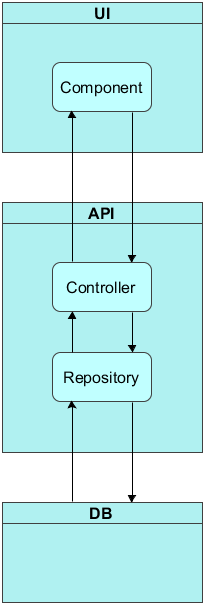
\includegraphics[scale=0.6]{images/architecture.png}
		\caption{Uproszczony schemat architektury z wyodrębnionymi najważniejszymi elementami składowymi.}
	\end{figure}
	
	
	System został zaprojektowany tak, by mógł zostać zintegrowany z istniejącymi zasobami firmy — jedyne dane, jakie przechowuje, dotyczą logiki biznesowej, związanej z wymaganiami funkcjonalnymi; wynika to z faktu, że większość firm ma już własne bazy danych przechowujące informacje o pracownikach więc duplikacja danych jest niepożądana ze względu na zużycie zasobów oraz możliwe problemy z synchronizacją. Dane związane z użytkownikami (np. imię, nazwisko, e-mail i numer telefonu) czy lokacjami firmy (np. adres) mogą zostać pobrane z innej bazy danych; ponadto interfejs użytkownika nie umożliwia wprowadzania lub edycji takich danych. Implementacja opisana w dalszej części niniejszej pracy przechowuje przykładowe dane użytkowników do celów testowych w tej samej bazie danych, jednakże konfiguracja systemu tak by korzystał z innej, nie stanowi większego problemu.
	
	W architekturze można rozróżnić trzy najważniejsze składowe, dwie pierwsze w interfejsie programistycznym i trzecią w interfejsie użytkownika:
	\begin{itemize}
		\item Kontroler (\textit{Controller}) to klasa odpowiadająca za obsługę żądań \textit{HTTP} \cite{msdn-aspnet-api}.
		\item Repozytorium (\textit{Repository}) zawiera logikę pośredniczącą w komunikacji między \textit{API} a bazą danych.
		\item Komponent (\textit{Component}) to podstawowy element definiujący działanie widoku w \textit{Angular} \cite{angular-components}.
	\end{itemize}
	
	\section{Standardy}
	Projekt był tworzony zgodnie z dobrymi praktykami programowania, z naciskiem na poprawną implementację obiektowego paradygmatu programowania. Interfejs programistyczny był tworzony z użyciem sztandarowych możliwości języka C\# takimi jak typy ogólne \cite{msdn-generics} (\textit{Generics}) pozwalające na tworzenie pojedynczych metod i klas zdolnych do operacji na wielu typach, zachowując wszystkie zalety silnego, statycznego typowania i wysoką wydajność.
	
	W celu zapewnienia przejrzystości kodu, nazewnictwo wszystkich elementów oraz dokumentacja kodu są zgodne ze standardową konwencją danego języka. Kod jest napisany w całości w języku angielskim.
	\begin{table}[H]
		\begin{tabularx}{\textwidth}{|l|l|l|l|X|}
			\hline
			Język      & Typy       			& Pliki                 & Zmienne prywatne & Inne zmienne \\ \hline
			C\# \cite{msdn-gnc}     & PascalCase & PascalCase.cs   		& camelCase        & PascalCase   \\ \hline
			TypeScript \cite{angular-sg} & PascalCase & snake-case.typ.ts 	& camelCase        & camelCase    \\ \hline
		\end{tabularx}
		\caption{Najważniejsze konwencje nazewnicze.}
	\end{table}
	
	\section{Przypadki użycia}
	
	
	
	\begin{figure}[h]
		\centering
		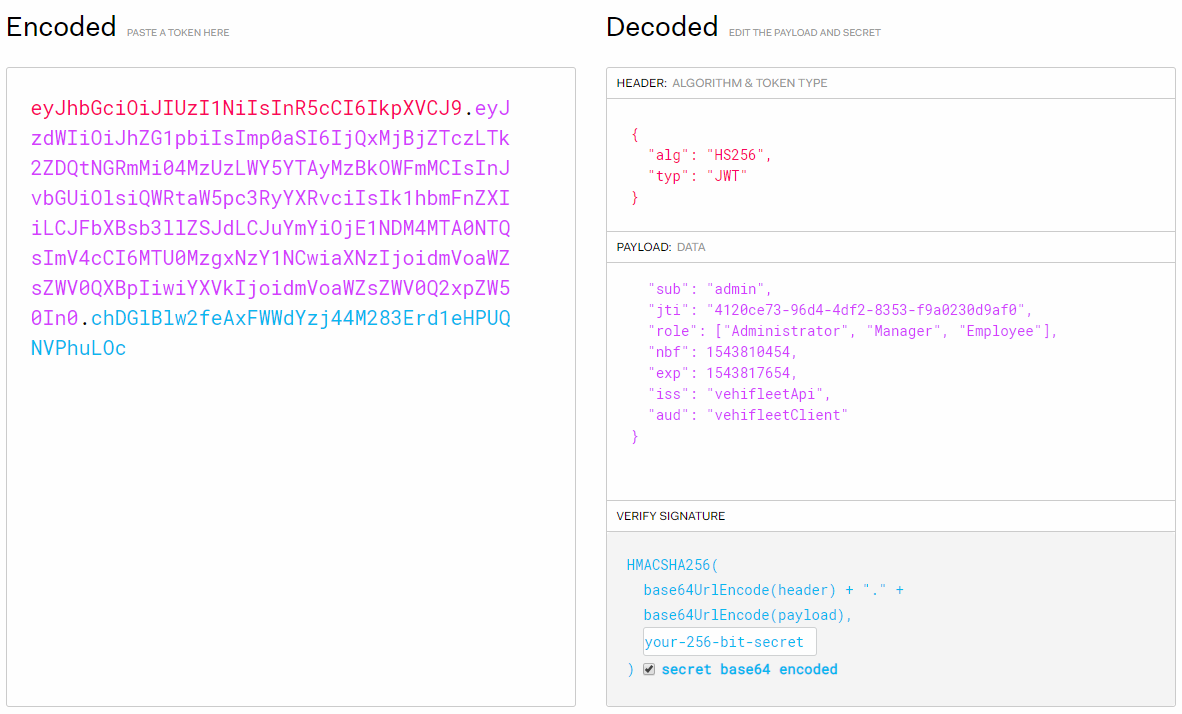
\includegraphics[scale=0.54]{images/jwt.png}
		\caption{Przykładowy token \textit{JWT}.}
		\small 
		Token został wygenerowany przy użyciu narzędzia ze strony \textit{https://jwt.io/}.
	\end{figure}
	
	\begin{table}[H]
		\caption{Domyślna konfiguracja relacji ról do poziomu uprawnień.}
		\begin{tabularx}{\textwidth}{|l|l|X|}
			\hline
			\multicolumn{1}{|c|}{\textbf{Aktor}} & \multicolumn{1}{c|}{\textbf{Poziom dostępu}} & \multicolumn{1}{c|}{\textbf{Wymagane role}} \\ \hline
			Kierowca                             & Podstawowy                                   & Employee                                    \\ \hline
			Kierownik                            & Pełny                                        & Manager lub Administrator                   \\ \hline
		\end{tabularx}
	\end{table}
	
	\newpage
	\section{Interfejs programistyczny}
	\subsection{Logika biznesowa}
	
	\begin{table}[H]
		\caption{Klasy obiektów biznesowych.}
		\begin{tabularx}{\textwidth}{|l|X|}
			\hline
			\textbf{Klasa}   & \textbf{Opis}                                                                                              \\ \hline
			VehicleModel     & Specyfikacja techniczna wspólna dla wielu pojazdów                                                         \\ \hline
			Vehicle          & Informacje unikatowe dla pewnego pojazdu                                                                   \\ \hline
			Insurance        & Ubezpieczenie                                                                                              \\ \hline
			Maintenance      & Naprawa, serwis pojazdu                                                                                    \\ \hline
			Employee         & Klasa używana do powiązania logiki biznesowej z informacjami o pracowniku                                  \\ \hline
			EmployeeIdentity & Dane personalne użytkownika; mogą być pobierane z innej bazy danych                                        \\ \hline
			Booking          & Rezerwacja pojazdu                                                                                         \\ \hline
			Location         & Informacje o budynkach należących do firmy korzystającej z systemu; mogą być pobierane z innej bazy danych \\ \hline
		\end{tabularx}
	\end{table}
	Baza danych została automatycznie wygenerowana na podstawie klas opisujących świat biznesowy, przy użyciu \textit{EF Core}. 
	
	Do zdefiniowania relacji między tabelami należy użyć pól typu takiego samego jak \textit{PK} docelowej klasy\cite{msdn-efcore-relationships}. Używanie adnotacji nie jest wymagane, o ile pole zostało nazwane według standardowej konwencji \textit{EF Core} — \textit{NazwaKlasyId} (np. \textit{VehicleId}). Dodatkowo klasę można uzupełnić o pola nawigacyjne (\textit{navigation properties}), pozwalające na odnoszenie się do powiązanej klasy w łatwy sposób w kodzie programu, należy jednak pamiętać że domyślnie \textit{EF Core 2.1} nie wczytuje informacji o powiązanych obiektach; podczas komunikacji z bazą daną należy jawnie wywołać ładowanie powiązanych obiektów za pomocą metody \textit{LINQ} \text{Include()}.
	
	Definiowanie właściwości kolumn wygenerowanych w bazie odbywa się poprzez umieszczenie odpowiednich adnotacji przy polach:
	\begin{itemize}
		\item $[$Key$]$: klucz główny (\textit{PK})
		\item $[$Required$]$: pole jest wymagane, nie może być puste (null)
	\end{itemize}
	
	\lstinputlisting[language=C,frame=single,caption=Przykład definiowania relacji między klasami w code-first]{source/efcore-model.cs}
	
	\lstinputlisting[language=C,frame=single,caption=Ładowanie powiązanych obiektów na przykładzie relacji rezerwacji do pojazdu]{source/efcore-loading-related.cs}
	
	\newpage 
	\begin{figure}[H]
		\centering
		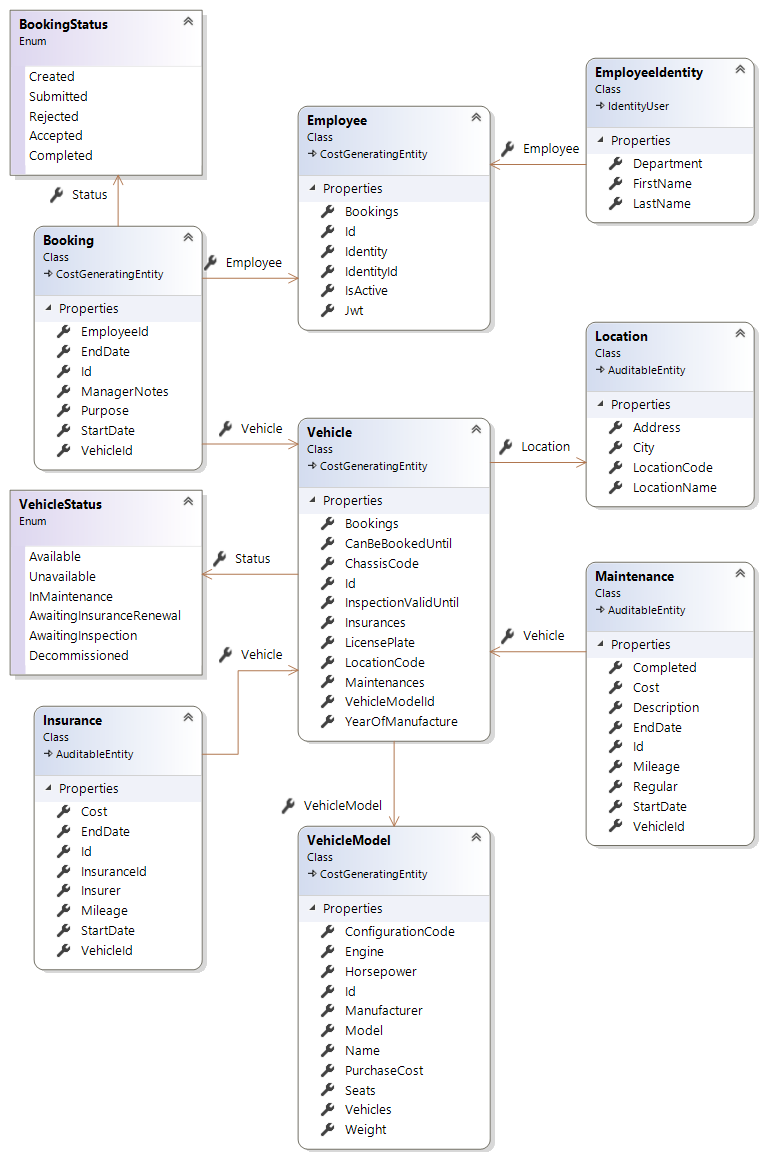
\includegraphics[width=\textwidth]{images/vs_class_diagram.png}
		\caption{Diagram klas.}
		\small 
		Diagram klas został wygenerowany przy użyciu \textit{Visual Studio}.
	\end{figure}
	
	\newpage 
	Wszystkie klasy związane z logiką biznesową dziedziczą po klasie \textit{AuditableEntity} posiadającej pola przechowujące informacje (data i nazwa użytkownika) o utworzeniu i ostatniej edycji encji. Klasy związane z elementami generującymi koszty (pojazdami, modelami pojazdów, rezerwacjimi i użytkownikami) dodatkowo dziedziczą po klasie \textit{CostGeneratingEntity} przechowującej informacje o koszcie, zużytym paliwie i przejechanych kilometrach. 
	
	Wybrana strategia dziedziczenia to \textit{TPC — Table per Concrete Type}. W strategii \textit{TPC} tabele utworzone w bazie danych zawierają wszystkie kolumny odpowiadające polom wszystkich klas w hierarchii dziedziczenia.
	
	\lstinputlisting[language=C,frame=single,caption=Klasa abstrakcyjna AuditableEntity]{source/efcore-auditable.cs}
	
	\lstinputlisting[language=C,frame=single,caption=Klasa abstrakcyjna CostGeneratingEntity]{source/efcore-costgenerating.cs}
	
	\subsection{Kontrolery}
	
	%----------------------------------------------------------------------------------------
	\begin{table}[H]
		\caption{Endpoint \textit{api/vehicle-models}.}
		\begin{tabularx}{\textwidth}{|l|l|X|}
			\hline
			\multicolumn{3}{|c|}{Opis}
			\\ \hline
			URL                         & \multicolumn{2}{l|}{api/vehicle-models}
			\\ \hline
			Wymagane role               & \multicolumn{2}{l|}{Employee}
			\\ \hline
			Metoda                      & \multicolumn{2}{l|}{GET}
			\\ \hline
			\multicolumn{3}{|c|}{ Odpowiedzi}
			\\ \hline
			\multirow{2}{*}{200 (OK)}   & Zawartość         & Tablica \textit{JSON}
			\\ \cline{2-3}              & Opis         	    & Lista modeli pojazdów
			\\ \hline
		\end{tabularx}
	\end{table}
	
	\begin{table}[H]
		\caption{Endpoint \textit{api/vehicle-models/manufacturers GET}.}
		\begin{tabularx}{\textwidth}{|l|l|X|}
			\hline
			\multicolumn{3}{|c|}{Opis}
			
			\\ \hline
			URL                         & \multicolumn{2}{l|}{api/vehicle-models/manufacturers}
			\\ \hline
			Wymagane role               & \multicolumn{2}{l|}{Employee}
			\\ \hline
			Metoda                      & \multicolumn{2}{l|}{GET}
			\\ \hline
			\multicolumn{3}{|c|}{Odpowiedzi}
			\\ \hline
			\multirow{2}{*}{200 (OK)}   & Zawartość        & Tablica \textit{JSON}
			\\ \cline{2-3}              & Opis         	   & Lista marek pojazdów
			\\ \hline
		\end{tabularx}
	\end{table}
	
	\begin{table}[H]
		\caption{Endpoint \textit{api/vehicle-models/id GET}.}
		\begin{tabularx}{\textwidth}{|l|l|X|}
			\hline
			\multicolumn{3}{|c|}{Opis}
			\\ \hline
			URL                         & \multicolumn{2}{l|}{api/vehicle-models/id}
			\\ \hline
			Wymagane role               & \multicolumn{2}{l|}{Employee}
			\\ \hline
			Metoda                      & \multicolumn{2}{l|}{GET}
			\\ \hline
			\multicolumn{3}{|c|}{Odpowiedzi}
			\\ \hline
			\multirow{2}{*}{200 (OK)} 	        & Zawartość   	& \textit{JSON}
			\\ \cline{2-3}                      & Opis         	& Model pojazdu o żądanym \textit{id}
			\\ \hline
			\multirow{2}{*}{404 (Not Found)} 	& Zawartość     & \lstinputlisting[language=json,nolol=true]{source/vehicle-models-get-by-id-404.json}
			\\ \cline{2-3}                      & Opis          & Model pojazdu o żądanym \textit{id} nie istnieje
			\\ \hline
		\end{tabularx}
	\end{table}
	
	\begin{table}[H]
		\caption{Endpoint \textit{api/vehicle-models POST}.}
		\begin{tabularx}{\textwidth}{|l|l|X|}
			\hline
			\multicolumn{3}{|c|}{Opis}
			\\ \hline
			URL                       & \multicolumn{2}{l|}{api/vehicle-models}
			\\ \hline
			Wymagane role             & \multicolumn{2}{l|}{Manager, Administrator}
			\\ \hline
			Metoda                    & \multicolumn{2}{l|}{POST}
			\\ \hline
			\multicolumn{3}{|c|}{Odpowiedzi}
			\\ \hline
			\multirow{2}{*}{200 (OK)} 		& Zawartość     & \textit{Id} utworzonego modelu pojazdu
			\\ \cline{2-3}                  & Opis         	& Model pojazdu został utworzony
			\\ \hline
		\end{tabularx}
	\end{table}
	
	\begin{table}[H]
		\caption{Endpoint \textit{api/vehicle-models/id PUT}.}
		\begin{tabularx}{\textwidth}{|l|l|X|}
			\hline
			\multicolumn{3}{|c|}{Opis}
			\\ \hline
			URL                       & \multicolumn{2}{l|}{api/vehicle-models/id}
			\\ \hline
			Wymagane role             & \multicolumn{2}{l|}{Manager, Administrator}
			\\ \hline
			Metoda                    & \multicolumn{2}{l|}{PUT}
			\\ \hline
			\multicolumn{3}{|c|}{Odpowiedzi}
			\\ \hline
			200 (OK) 		 & Opis      	& Model pojazdu został zaktualizowany
			\\ \hline
			\multirow{2}{*}{404 (Not Found)} 	    & Zawartość     & \lstinputlisting[language=json,nolol=true]{source/vehicle-models-put-404.json}  
			\\ \cline{2-3}                          & Opis          & Model pojazdu o żądanym \textit{id} nie istnieje
			\\ \hline
		\end{tabularx}
	\end{table}
	
	\begin{table}[H]
		\caption{Endpoint \textit{api/vehicle-models/id DELETE}.}
		\begin{tabularx}{\textwidth}{|l|l|X|}
			\hline
			\multicolumn{3}{|c|}{Opis}
			\\ \hline
			URL                       & \multicolumn{2}{l|}{api/vehicle-models/id}
			\\ \hline
			Wymagane role             & \multicolumn{2}{l|}{Manager, Administrator}
			\\ \hline
			Metoda                    & \multicolumn{2}{l|}{DELETE}
			\\ \hline
			\multicolumn{3}{|c|}{Odpowiedzi}
			\\ \hline
			200 (OK)			                & Opis         	& Model pojazdu został usunięty
			\\ \hline
			\multirow{2}{*}{404 (Not Found)} 	& Zawartość     & \lstinputlisting[language=json,nolol=true]{source/vehicle-models-delete-404.json}   	
			\\ \cline{2-3}                      & Opis          & Model pojazdu o żądanym \textit{id} nie istnieje
			\\ \hline
			\multirow{2}{*}{400 (Bad Request)} 	& Zawartość     & \lstinputlisting[language=json,nolol=true]{source/vehicle-models-delete-400.json}   	
			\\ \cline{2-3}                      & Opis          & System posiada egzemplarze modelu pojazdu o żądanym \textit{id}, nie może on zostać usunięty
			\\ \hline
		\end{tabularx}
	\end{table}
	
	%----------------------------------------------------------------------------------------
	\newpage
	\begin{table}[H]
		\caption{Endpoint \textit{api/vehicles}.}
		\begin{tabularx}{\textwidth}{|l|l|X|}
			\hline
			\multicolumn{3}{|c|}{Opis}
			\\ \hline
			URL                         & \multicolumn{2}{l|}{api/vehicles}
			\\ \hline
			Wymagane role               & \multicolumn{2}{l|}{Employee}
			\\ \hline
			Metoda                      & \multicolumn{2}{l|}{GET}
			\\ \hline
			\multicolumn{3}{|c|}{ Odpowiedzi}
			\\ \hline
			\multirow{2}{*}{200 (OK)}   & Zawartość         & Tablica \textit{JSON}
			\\ \cline{2-3}              & Opis         	    & Lista pojazdów
			\\ \hline
		\end{tabularx}
	\end{table}
	
	\begin{table}[H]
		\caption{Endpoint \textit{api/vehicles/id GET}.}
		\begin{tabularx}{\textwidth}{|l|l|X|}
			\hline
			\multicolumn{3}{|c|}{Opis}
			\\ \hline
			URL                         & \multicolumn{2}{l|}{api/vehicles/id}
			\\ \hline
			Wymagane role               & \multicolumn{2}{l|}{Employee}
			\\ \hline
			Metoda                      & \multicolumn{2}{l|}{GET}
			\\ \hline
			\multicolumn{3}{|c|}{Odpowiedzi}
			\\ \hline
			\multirow{2}{*}{200 (OK)} 	        & Zawartość   	& \textit{JSON}
			\\ \cline{2-3}                      & Opis         	& Pojazd o żądanym \textit{id}
			\\ \hline
			\multirow{2}{*}{404 (Not Found)} 	& Zawartość     & \lstinputlisting[language=json,nolol=true]{source/vehicles-get-by-id-404.json}
			\\ \cline{2-3}                      & Opis          & Pojazd o żądanym \textit{id} nie istnieje
			\\ \hline
		\end{tabularx}
	\end{table}
	
	\begin{table}[H]
		\caption{Endpoint \textit{api/vehicles POST}.}
		\begin{tabularx}{\textwidth}{|l|l|X|}
			\hline
			\multicolumn{3}{|c|}{Opis}
			\\ \hline
			URL                       & \multicolumn{2}{l|}{api/vehicles}
			\\ \hline
			Wymagane role             & \multicolumn{2}{l|}{Manager, Administrator}
			\\ \hline
			Metoda                    & \multicolumn{2}{l|}{POST}
			\\ \hline
			\multicolumn{3}{|c|}{Odpowiedzi}
			\\ \hline
			\multirow{2}{*}{200 (OK)} 		& Zawartość     & \textit{Id} utworzonego pojazdu
			\\ \cline{2-3}                  & Opis         	& Pojazd został utworzony
			\\ \hline
		\end{tabularx}
	\end{table}
	
	\begin{table}[H]
		\caption{Endpoint \textit{api/vehicles/id PUT}.}
		\begin{tabularx}{\textwidth}{|l|l|X|}
			\hline
			\multicolumn{3}{|c|}{Opis}
			\\ \hline
			URL                       & \multicolumn{2}{l|}{api/vehicles/id}
			\\ \hline
			Wymagane role             & \multicolumn{2}{l|}{Manager, Administrator}
			\\ \hline
			Metoda                    & \multicolumn{2}{l|}{PUT}
			\\ \hline
			\multicolumn{3}{|c|}{Odpowiedzi}
			\\ \hline
			200 (OK) 		                        & Opis      	& Pojazd zostało zaktualizowane
			\\ \hline
			\multirow{2}{*}{404 (Not Found)} 	    & Zawartość     & \lstinputlisting[language=json,nolol=true]{source/vehicles-put-404.json}  
			\\ \cline{2-3}                          & Opis          & Pojazd o żądanym \textit{id} nie istnieje
			\\ \hline
		\end{tabularx}
	\end{table}
	
	\begin{table}[H]
		\caption{Endpoint \textit{api/vehicles/id DELETE}.}
		\begin{tabularx}{\textwidth}{|l|l|X|}
			\hline
			\multicolumn{3}{|c|}{Opis}
			\\ \hline
			URL                       & \multicolumn{2}{l|}{api/vehicles/id}
			\\ \hline
			Wymagane role             & \multicolumn{2}{l|}{Manager, Administrator}
			\\ \hline
			Metoda                    & \multicolumn{2}{l|}{DELETE}
			\\ \hline
			\multicolumn{3}{|c|}{Odpowiedzi}
			\\ \hline
			200 (OK)			                & Opis         	& Pojazd został usunięty
			\\ \hline
			\multirow{2}{*}{404 (Not Found)} 	& Zawartość     & \lstinputlisting[language=json,nolol=true]{source/vehicles-delete-404.json}   	
			\\ \cline{2-3}                      & Opis          & Pojazd o żądanym \textit{id} nie istnieje
			\\ \hline
			\multirow{2}{*}{400 (Bad Request)} 	& Zawartość     & \lstinputlisting[language=json,nolol=true]{source/vehicles-delete-400.json}   	
			\\ \cline{2-3}                      & Opis          & System posiada rezerwacje przypisane do pojazdu o żądanym \textit{id}, nie może on zostać usunięty
			\\ \hline
		\end{tabularx}
	\end{table}
	
	%----------------------------------------------------------------------------------------
	\begin{table}[H]
		\caption{Endpoint \textit{api/insurances/vehicle/id}.}
		\begin{tabularx}{\textwidth}{|l|l|X|}
			\hline
			\multicolumn{3}{|c|}{Opis}
			\\ \hline
			URL                         & \multicolumn{2}{l|}{api/insurances}
			\\ \hline
			Wymagane role               & \multicolumn{2}{l|}{Employee}
			\\ \hline
			Metoda                      & \multicolumn{2}{l|}{GET}
			\\ \hline
			\multicolumn{3}{|c|}{ Odpowiedzi}
			\\ \hline
			\multirow{2}{*}{200 (OK)}   & Zawartość         & Tablica \textit{JSON}
			\\ \cline{2-3}              & Opis         	    & Lista ubezpieczeń przypisanych do danego pojazdu
			\\ \hline
		\end{tabularx}
	\end{table}
	
	\begin{table}[H]
		\caption{Endpoint \textit{api/insurances/id GET}.}
		\begin{tabularx}{\textwidth}{|l|l|X|}
			\hline
			\multicolumn{3}{|c|}{Opis}
			\\ \hline
			URL                         & \multicolumn{2}{l|}{api/insurances/id}
			\\ \hline
			Wymagane role               & \multicolumn{2}{l|}{Employee}
			\\ \hline
			Metoda                      & \multicolumn{2}{l|}{GET}
			\\ \hline
			\multicolumn{3}{|c|}{Odpowiedzi}
			\\ \hline
			\multirow{2}{*}{200 (OK)} 	        & Zawartość   	& \textit{JSON}
			\\ \cline{2-3}                      & Opis         	& Ubezpieczenie o żądanym \textit{id}
			\\ \hline
			\multirow{2}{*}{404 (Not Found)} 	& Zawartość     & \lstinputlisting[language=json,nolol=true]{source/insurances-get-by-id-404.json}
			\\ \cline{2-3}                      & Opis          & Ubezpieczenie o żądanym \textit{id} nie istnieje
			\\ \hline
		\end{tabularx}
	\end{table}
	
	\begin{table}[H]
		\caption{Endpoint \textit{api/insurances POST}.}
		\begin{tabularx}{\textwidth}{|l|l|X|}
			\hline
			\multicolumn{3}{|c|}{Opis}
			\\ \hline
			URL                       & \multicolumn{2}{l|}{api/insurances}
			\\ \hline
			Wymagane role             & \multicolumn{2}{l|}{Manager, Administrator}
			\\ \hline
			Metoda                    & \multicolumn{2}{l|}{POST}
			\\ \hline
			\multicolumn{3}{|c|}{Odpowiedzi}
			\\ \hline
			\multirow{2}{*}{200 (OK)} 		& Zawartość     & \textit{Id} utworzonego ubezpieczenia
			\\ \cline{2-3}                  & Opis         	& Ubezpieczenie został utworzony
			\\ \hline
		\end{tabularx}
	\end{table}
	
	\begin{table}[H]
		\caption{Endpoint \textit{api/insurances/id PUT}.}
		\begin{tabularx}{\textwidth}{|l|l|X|}
			\hline
			\multicolumn{3}{|c|}{Opis}
			\\ \hline
			URL                       & \multicolumn{2}{l|}{api/insurances/id}
			\\ \hline
			Wymagane role             & \multicolumn{2}{l|}{Manager, Administrator}
			\\ \hline
			Metoda                    & \multicolumn{2}{l|}{PUT}
			\\ \hline
			\multicolumn{3}{|c|}{Odpowiedzi}
			\\ \hline
			200 (OK) 		                        & Opis      	& Ubezpieczenie zostało zaktualizowane
			\\ \hline
			\multirow{2}{*}{404 (Not Found)} 	    & Zawartość     & \lstinputlisting[language=json,nolol=true]{source/insurances-put-404.json}
			\\ \cline{2-3}                          & Opis          & Ubezpieczenie o żądanym \textit{id} nie istnieje
			\\ \hline
		\end{tabularx}
	\end{table}
	
	\begin{table}[H]
		\caption{Endpoint \textit{api/insurances/id DELETE}.}
		\begin{tabularx}{\textwidth}{|l|l|X|}
			\hline
			\multicolumn{3}{|c|}{Opis}
			\\ \hline
			URL                       & \multicolumn{2}{l|}{api/insurances/id}
			\\ \hline
			Wymagane role             & \multicolumn{2}{l|}{Manager, Administrator}
			\\ \hline
			Metoda                    & \multicolumn{2}{l|}{DELETE}
			\\ \hline
			\multicolumn{3}{|c|}{Odpowiedzi}
			\\ \hline
			200 (OK)			                & Opis         	& Ubezpieczenie został usunięty
			\\ \hline
			\multirow{2}{*}{404 (Not Found)} 	& Zawartość     & \lstinputlisting[language=json,nolol=true]{source/insurances-delete-404.json}
			\\ \cline{2-3}                      & Opis          & Ubezpieczenie o żądanym \textit{id} nie istnieje
			\\ \hline
		\end{tabularx}
	\end{table}
	
	%----------------------------------------------------------------------------------------
	\begin{table}[H]
		\caption{Endpoint \textit{api/maintenances/vehicle/id}.}
		\begin{tabularx}{\textwidth}{|l|l|X|}
			\hline
			\multicolumn{3}{|c|}{Opis}
			\\ \hline
			URL                         & \multicolumn{2}{l|}{api/maintenances}
			\\ \hline
			Wymagane role               & \multicolumn{2}{l|}{Employee}
			\\ \hline
			Metoda                      & \multicolumn{2}{l|}{GET}
			\\ \hline
			\multicolumn{3}{|c|}{ Odpowiedzi}
			\\ \hline
			\multirow{2}{*}{200 (OK)}   & Zawartość         & Tablica \textit{JSON}
			\\ \cline{2-3}              & Opis         	    & Lista napraw przypisanych do danego pojazdu
			\\ \hline
		\end{tabularx}
	\end{table}
	
	\begin{table}[H]
		\caption{Endpoint \textit{api/maintenances/id GET}.}
		\begin{tabularx}{\textwidth}{|l|l|X|}
			\hline
			\multicolumn{3}{|c|}{Opis}
			\\ \hline
			URL                         & \multicolumn{2}{l|}{api/maintenances/id}
			\\ \hline
			Wymagane role               & \multicolumn{2}{l|}{Employee}
			\\ \hline
			Metoda                      & \multicolumn{2}{l|}{GET}
			\\ \hline
			\multicolumn{3}{|c|}{Odpowiedzi}
			\\ \hline
			\multirow{2}{*}{200 (OK)} 	        & Zawartość   	& \textit{JSON}
			\\ \cline{2-3}                      & Opis         	& Naprawa o żądanym \textit{id}
			\\ \hline
			\multirow{2}{*}{404 (Not Found)} 	& Zawartość     & \lstinputlisting[language=json,nolol=true]{source/maintenances-get-by-id-404.json}
			\\ \cline{2-3}                      & Opis          & Naprawa o żądanym \textit{id} nie istnieje
			\\ \hline
		\end{tabularx}
	\end{table}
	
	\begin{table}[H]
		\caption{Endpoint \textit{api/maintenances POST}.}
		\begin{tabularx}{\textwidth}{|l|l|X|}
			\hline
			\multicolumn{3}{|c|}{Opis}
			\\ \hline
			URL                       & \multicolumn{2}{l|}{api/maintenances}
			\\ \hline
			Wymagane role             & \multicolumn{2}{l|}{Manager, Administrator}
			\\ \hline
			Metoda                    & \multicolumn{2}{l|}{POST}
			\\ \hline
			\multicolumn{3}{|c|}{Odpowiedzi}
			\\ \hline
			\multirow{2}{*}{200 (OK)} 		& Zawartość     & \textit{Id} utworzonego ubezpieczenia
			\\ \cline{2-3}                  & Opis         	& Naprawa została utworzona
			\\ \hline
		\end{tabularx}
	\end{table}
	
	\begin{table}[H]
		\caption{Endpoint \textit{api/maintenances/id PUT}.}
		\begin{tabularx}{\textwidth}{|l|l|X|}
			\hline
			\multicolumn{3}{|c|}{Opis}
			\\ \hline
			URL                       & \multicolumn{2}{l|}{api/maintenances/id}
			\\ \hline
			Wymagane role             & \multicolumn{2}{l|}{Manager, Administrator}
			\\ \hline
			Metoda                    & \multicolumn{2}{l|}{PUT}
			\\ \hline
			\multicolumn{3}{|c|}{Odpowiedzi}
			\\ \hline
			200 (OK) 		                        & Opis      	& Naprawa została zauktualizowana
			\\ \hline
			\multirow{2}{*}{404 (Not Found)} 	    & Zawartość     & \lstinputlisting[language=json,nolol=true]{source/maintenances-put-404.json}
			\\ \cline{2-3}                          & Opis          & Naprawa o żądanym \textit{id} nie istnieje
			\\ \hline
		\end{tabularx}
	\end{table}
	
	\begin{table}[H]
		\caption{Endpoint \textit{api/maintenances/id DELETE}.}
		\begin{tabularx}{\textwidth}{|l|l|X|}
			\hline
			\multicolumn{3}{|c|}{Opis}
			\\ \hline
			URL                       & \multicolumn{2}{l|}{api/maintenances/id}
			\\ \hline
			Wymagane role             & \multicolumn{2}{l|}{Manager, Administrator}
			\\ \hline
			Metoda                    & \multicolumn{2}{l|}{DELETE}
			\\ \hline
			\multicolumn{3}{|c|}{Odpowiedzi}
			\\ \hline
			200 (OK)			                & Opis         	& Naprawa została usunięta
			\\ \hline
			\multirow{2}{*}{404 (Not Found)} 	& Zawartość     & \lstinputlisting[language=json,nolol=true]{source/maintenances-delete-404.json}
			\\ \cline{2-3}                      & Opis          & Naprawa o żądanym \textit{id} nie istnieje
			\\ \hline
		\end{tabularx}
	\end{table}
	
	%----------------------------------------------------------------------------------------
	\begin{table}[H]
		\caption{Endpoint \textit{api/bookings/vehicle/id}.}
		\begin{tabularx}{\textwidth}{|l|l|X|}
			\hline
			\multicolumn{3}{|c|}{Opis}
			\\ \hline
			URL                         & \multicolumn{2}{l|}{api/bookings}
			\\ \hline
			Wymagane role               & \multicolumn{2}{l|}{Employee}
			\\ \hline
			Metoda                      & \multicolumn{2}{l|}{GET}
			\\ \hline
			\multicolumn{3}{|c|}{ Odpowiedzi}
			\\ \hline
			\multirow{2}{*}{200 (OK)}   & Zawartość         & Tablica \textit{JSON}
			\\ \cline{2-3}              & Opis         	    & Lista rezerwacji
			\\ \hline
		\end{tabularx}
	\end{table}
	
	\begin{table}[H]
		\caption{Endpoint \textit{api/bookings/id GET}.}
		\begin{tabularx}{\textwidth}{|l|l|X|}
			\hline
			\multicolumn{3}{|c|}{Opis}
			\\ \hline
			URL                         & \multicolumn{2}{l|}{api/bookings/id}
			\\ \hline
			Wymagane role               & \multicolumn{2}{l|}{Employee}
			\\ \hline
			Metoda                      & \multicolumn{2}{l|}{GET}
			\\ \hline
			\multicolumn{3}{|c|}{Odpowiedzi}
			\\ \hline
			\multirow{2}{*}{200 (OK)} 	        & Zawartość   	& \textit{JSON}
			\\ \cline{2-3}                      & Opis         	& Rezerwacja o żądanym \textit{id}
			\\ \hline
			\multirow{2}{*}{404 (Not Found)} 	& Zawartość     & \lstinputlisting[language=json,nolol=true]{source/booking-get-by-id-404.json}
			\\ \cline{2-3}                      & Opis          & Rezerwacja o żądanym \textit{id} nie istnieje
			\\ \hline
		\end{tabularx}
	\end{table}
	
	\begin{table}[H]
		\caption{Endpoint \textit{api/bookings POST}.}
		\begin{tabularx}{\textwidth}{|l|l|X|}
			\hline
			\multicolumn{3}{|c|}{Opis}
			\\ \hline
			URL                       & \multicolumn{2}{l|}{api/bookings}
			\\ \hline
			Wymagane role             & \multicolumn{2}{l|}{Manager, Administrator}
			\\ \hline
			Metoda                    & \multicolumn{2}{l|}{POST}
			\\ \hline
			\multicolumn{3}{|c|}{Odpowiedzi}
			\\ \hline
			\multirow{2}{*}{200 (OK)} 		& Zawartość     & \textit{Id} utworzonej rezerwacji
			\\ \cline{2-3}                  & Opis         	& Rezerwacja została utworzona
			\\ \hline
			\multirow{2}{*}{400 (Bad Request)} 	& Zawartość     &  \lstinputlisting[language=json,nolol=true]{source/booking-post-400-1.json}  
			\\ \cline{2-3}                      & Opis          & Pracownik powiązany z rezerwacją nie istnieje      						    
			\\ \hline
			\multirow{2}{*}{400 (Bad Request)} 	& Zawartość     &  \lstinputlisting[language=json,nolol=true]{source/booking-post-400-2.json}  
			\\ \cline{2-3}                      & Opis          & Pojazd powiązany z rezerwacją nie istnieje      								
			\\ \hline      
		\end{tabularx}
	\end{table}
	
	\begin{table}[H]
		\caption{Endpoint \textit{api/bookings/id PUT}.}
		\begin{tabularx}{\textwidth}{|l|l|X|}
			\hline
			\multicolumn{3}{|c|}{Opis}
			\\ \hline
			URL                       & \multicolumn{2}{l|}{api/bookings/id}
			\\ \hline
			Wymagane role             & \multicolumn{2}{l|}{Employee}
			\\ \hline
			Metoda                    & \multicolumn{2}{l|}{PUT}
			\\ \hline
			\multicolumn{3}{|c|}{Odpowiedzi}
			\\ \hline
			200 (OK) 		                        & Opis      	& Rezerwacja została zauktualizowana
			\\ \hline
			\multirow{2}{*}{404 (Not Found)} 	    & Zawartość     & \lstinputlisting[language=json,nolol=true]{source/booking-put-404.json}
			\\ \cline{2-3}                          & Opis          & Rezerwacja o żądanym \textit{id} nie istnieje
			\\ \hline
		\end{tabularx}
	\end{table}
	
	\begin{table}[H]
		\caption{Endpoint \textit{api/bookings/id DELETE}.}
		\begin{tabularx}{\textwidth}{|l|l|X|}
			\hline
			\multicolumn{3}{|c|}{Opis}
			\\ \hline
			URL                       & \multicolumn{2}{l|}{api/bookings/id}
			\\ \hline
			Wymagane role             & \multicolumn{2}{l|}{Employee}
			\\ \hline
			Metoda                    & \multicolumn{2}{l|}{DELETE}
			\\ \hline
			\multicolumn{3}{|c|}{Odpowiedzi}
			\\ \hline
			200 (OK)			                & Opis         	& Rezerwacja została usunięta
			\\ \hline
			\multirow{2}{*}{404 (Not Found)} 	& Zawartość     & \lstinputlisting[language=json,nolol=true]{source/booking-delete-404.json}
			\\ \cline{2-3}                      & Opis          & Rezerwacja o żądanym \textit{id} nie istnieje
			\\ \hline
		\end{tabularx}
	\end{table}
	%----------------------------------------------------------------------------------------
	
	
	\subsection{Filtrowanie wyników żądań GET}
	Interfejs programistyczny umożliwia filtrowanie wyników żądań \textit{GET} poprzez warunki przesyłane w \textit{URL}.
	
	Mechanizm filtrowania jest wydajny nawet dla skomplikowanych żądań - implementacja korzysta z interfejsu \textit{IQueryable}, pozwalającego na dodawanie wielu warunków które zostaną wykonane wyłącznie raz. W trakcie wywołania funkcji \textit{ToListAsync()}, warunki dodane do \textit{IQueryable} zostaną przetłumaczone do pojedynczego zapytania \textit{SQL} które zostanie wykonane w bazie danych po czym zwróci listę obiektów.
	
	\lstinputlisting[language=C,frame=single,caption=Logika filtrującą dla modeli pojazdów]{source/iqueryable-filter.cs}
	
	\begin{table}[H]
		\caption{Filtr modeli pojazdów (\textit{api/vehicle-models GET}).}
		\begin{tabularx}{\textwidth}{|l|X|}
			\hline                                       							
			\multicolumn{2}{|c|}{\textbf{Filtr modeli pojazdów}}  							        \\ \hline
			URL                 & api/vehicle-models     							             	\\ \hline
			\multicolumn{2}{|c|}{\textbf{Warunki}}     												\\ \hline
			\textbf{Nazwa}      & \textbf{Opis}              										\\ \hline
			Manufacturer        & Producent         												\\ \hline
			\multicolumn{2}{|c|}{\textbf{Przykładowy filtr}}										\\ \hline
			URL                 & api/vehicle-models?manufacturer=Ford								\\ \hline
			\multicolumn{2}{|l|}{API zwróci wyłącznie modele samochodów wyprodukowane przez Forda}	\\ \hline
		\end{tabularx}
	\end{table}
	
	\begin{table}[H]
		\caption{Filtr pojazdów (\textit{api/vehicles GET}).}
		\begin{tabularx}{\textwidth}{|l|X|}
			\hline                                       							
			\multicolumn{2}{|c|}{\textbf{Filtr modeli pojazdów}}  							        	\\ \hline
			URL                 & api/vehicle-models     							             		\\ \hline
			\multicolumn{2}{|c|}{\textbf{Warunki}}     													\\ \hline
			\textbf{Nazwa}      & \textbf{Opis}              											\\ \hline
			Manufacturer        & Producent         													\\ \hline
			VehicleModelId      & Id modelu	        													\\ \hline
			LocationCode        & Id obecnej lokalizacji												\\ \hline
			ChassisCode         & Kod karoserii 	  													\\ \hline
			MinBookingDays      & Minimalna ilość dni w których pojazd jest dostępny					\\ \hline
			Status              & Obecny status pojazdu         										\\ \hline										
			\multicolumn{2}{|c|}{\textbf{Przykładowy filtr}}											\\ \hline
			URL                 & api/vehicles?Manufacturer=Ford\&LocationCode=KRK-1\&MinBookingDays=30	\\ \hline
			\multicolumn{2}{|X|}{API zwróci wyłącznie samochodowy wyprodukowane przez Forda, przebywające w lokalizacji KRK-1 oraz dostępne na co najmniej 30 dni}		\\ \hline
		\end{tabularx}
	\end{table}
	
	\begin{table}[H]
		\caption{Filtr rezerwacji (\textit{api/bookings GET}).}
		\begin{tabularx}{\textwidth}{|l|X|}
			\hline                                       							
			\multicolumn{2}{|c|}{\textbf{Filtr rezerwacji}}							        		\\ \hline
			URL                 & api/bookings     							             			\\ \hline
			\multicolumn{2}{|c|}{\textbf{Warunki}}     												\\ \hline
			\textbf{Nazwa}      & \textbf{Opis}              										\\ \hline
			EmployeeId        	& Id pracownika który utworzył rezerwację 						    \\ \hline
			EmployeeUserName	& Nazwa użytkownika który utworzył rezerwację						\\ \hline	
			VehicleId	        & Id rezerwowanego pojazdu       									\\ \hline
			Statuses        	& Dozwolone statusy rezerwacji         							    \\ \hline
			FromDate       		& Data po której rozpoczęły się rezerwacji						    \\ \hline
			ToDate 			    & Data przed którą zakończyły się rezerwacji						\\ \hline											
			\multicolumn{2}{|c|}{\textbf{Przykładowy filtr}}										\\ \hline
			URL                 & api/bookings?Statuses=Completed\&Statuses=Rejected\&Em-ployeeUserName=jkowalski \\ \hline
			\multicolumn{2}{|X|}{API zwróci zakończone (\textit{Completed}) lub odrzucone (\textit{Rejected}) rezerwacji utworzone przez użytkownika jkowalski}	\\ \hline
		\end{tabularx}
	\end{table}
	
	\newpage
	\subsection{Eksport statystyk floty}
	System przechowuje informacje na temat bieżących kosztów generowanych przez flotę; raporty zawierające te informacje mogą być wyeksportowane do pliku \textit{.csv} by następnie zostać zaimportowane do narzędzia kalkulacyjnego, takiego jak \textit{Microsoft Excel}.
	
	W utworzonym systemie eksport do pliku wywoływany jest przez żądanie \textit{HTTP POST} na adres \textit{api/reports/generate/days}, gdzie \textit{days} to liczba określająca z jak wielu dni wstecz powinny być brane dane dotyczące rezerwacji.
	
	\lstinputlisting[frame=single,caption=Przykładowy raport ze statystykami pojazdów]{source/report.csv}
	\newpage
	
	
	
	\section{Interfejs użytkownika}
	\subsection{Układ interfejsu użytkownika}
	Komponenty (widoki) wchodzące w skład interfejsu użytkownika można podzielić na dwa główne rodzaje:
	\begin{itemize}
		\item \textbf{Widok szczegółowy} (\textit{detail}) który zawiera komplet informacji o danym obiekcie i umożliwia jego edycję.
		\item \textbf{Widok listy} (\textit{list}) zawierający małą ilość informacji wymaganych do identyfikacji danego obiektu oraz możliwość przejścia do \textbf{widoku szczegółowego}. Widoki tego typu są punktem wejściowym do bardziej zaawansowanej logiki interfejsu, dostępnym bezpośrednio za pomocą paska nawigacji (\textit{navbar}).
	\end{itemize}
	\begin{figure}[h]
		\centering
		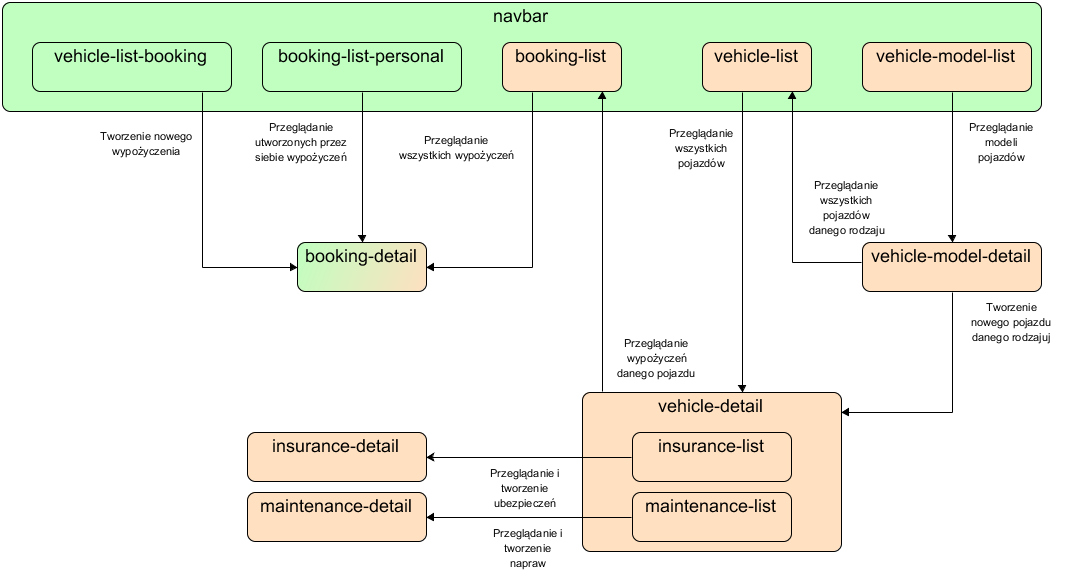
\includegraphics[scale=0.62]{images/angular_views.png}
		\caption{Widoki interfejsu użytkownika.}
		\small 
		Widoki zielone dostępne są dla każdego użytkownika; widoki pomarańczowe wyłącznie dla użytkownika o odpowiednich uprawnieniach. Widok \textit{booking-detail} jest specjalnym przypadkiem oferującym różne możliwości w zależności od uprawnień użytkownika.
	\end{figure}
	
	\section{Bezpieczeństwo}
	Dostęp do systemu został zabezpieczony przy użyciu standardu \textit{JSON Web Token (JWT)} \cite{jwt}. Autoryzacja \textit{JWT} bazuje na generowaniu podpisanych (przez co odpornych na sfałszowanie) tokenów po stronie interfejsu programistycznego, a następnie wysyłaniu ich do aplikacji klienta. \textit{API} wcześniej wygenerowanego wymaga tokena w nagłówku \textit{HTTP} dla każdego żądania wysłanego przez interfejs użytkownika; żądania z niepoprawnym tokenem zostają odrzucone.
	
	Schemat działania autoryzacji \textit{JWT} w opisywanym projekcie wygląda następująco:
	\begin{enumerate}
		\item Użytkownik loguje się przez interfejs użytkownika, podając nazwę użytkownika oraz hasło
		\item Interfejs programistyczny weryfikuje dane logowania
		\item W przypadku prawidłowego hasła utworzony zostaje token \textit{JWT} zawierający:
		\subitem Informacje o wydającym token
		\subitem Informacje o użytkowniku: jego identyfikator (nazwa użytkownika) oraz role
		\item Utworzony token zostaje zaszyfrowany (uniemożliwiając jego sfałszowanie) i zwrócony	
		\item Odebrany token zostaje umieszczony w pamięci przeglądarki internetowej użytkownika
	\end{enumerate}
	Interfejs programistyczny weryfikuje poprawność tokena dla każdego żądania \textit{HTTP} z wyjątkiem tych związanych z procesem autoryzacji użytkownika; jeżeli token jest niepoprawny lub zbyt stary (wydany więcej niż 2 godziny przed weryfikacją), żądanie jest odrzucone.
	
	Przechowywanie ról w tokenie \textit{JWT} pozwala na autoryzację z uwzględnieniem uprawnień użytkownika, przykładowo, ograniczając dostęp do poufnych informacji lub modyfikacji przechowywanych danych przez osoby nieuprawnione.
	
	
	%\section{Konteneryzacja}
	%----------------------------------------------------------------------------------------
	%	SECTION 6
	%----------------------------------------------------------------------------------------
	%\newpage
	%\chapter{Implementacja}
	
	%----------------------------------------------------------------------------------------
	%	SECTION 7
	%----------------------------------------------------------------------------------------
	\newpage
	\chapter{Testy}
	\section{Testy jednostkowe}
	System był testowany przy użyciu testów jednostkowych korzystających z biblioteki \textit{XUnit} oraz napisanych w schludny, zgodny z często stosowaną w języku C\# konwencją \textit{AAA} sposób, bazujący na podziale testu na trzy sekcje:
	\begin{enumerate}
		\item Przygotuj (\textit{Arrange}): przygotowanie niezbędnych zmiennych
		\item Działaj (\textit{Act}): wywołanie metod które mają być testowane 
		\item Sprawdź (\textit{Assert}): sprawdzenie wyniku 
	\end{enumerate}
	
	\lstinputlisting[language=C,frame=single,caption=Przykład testu jednostkowego zgodnego z konwencją \textit{AAA}]{source/tests-unit.cs}
	
	\section{Testy systemowe}
	Najczęściej stosowanym rodzajem testów były testy systemowe przy użyciu narzędzia \textit{Postman} pozwalającego na wygodne tworzenie i wysyłanie skomplikowanych żądań \textit{HTTP}. \textit{Postman} pozwala również na zapisywanie oraz organizowanie żądań co znacznie przyśpiesza proces testowania.
	\begin{figure}[H]
		\centering
		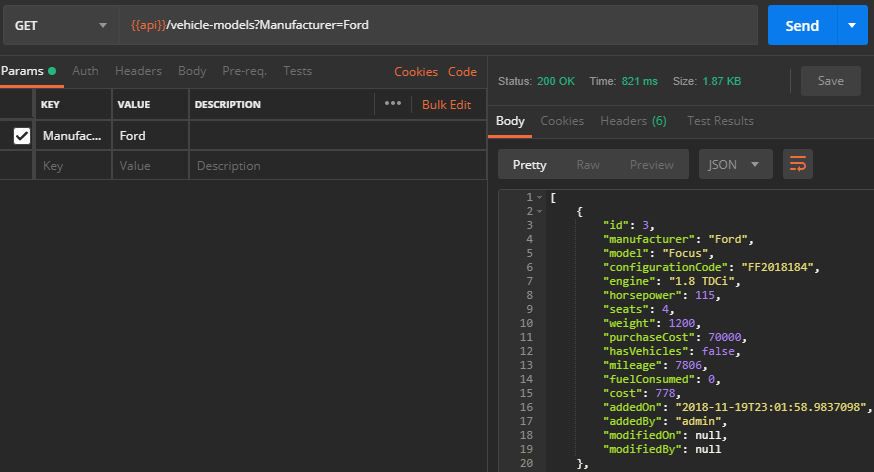
\includegraphics[width=\textwidth]{images/tests_postman.png}
		\caption{Interfejs programu Postman.}
	\end{figure}
	\section{Testy dymne}
	Testy dymne (\textit{smoke test}) były używane w końcowej fazie projektu; polegały na wcieleniu się w rolę użytkownika i przechodzeniu najczęściej używanych ścieżek (np. tworzeniu rezerwacji) . Testy tego typu pozwalają szybko zweryfikować czy kluczowa funkcjonalność systemu działa bezproblemowo.
	
	%----------------------------------------------------------------------------------------
	%	SECTION 8
	%----------------------------------------------------------------------------------------
	\newpage
	\chapter{Podsumowanie}
	\section{Wnioski}
	Celem pracy było utworzenie systemu pozwalającego na kontrolę dostępu do pojazdów oraz śledzeniu ich stanu; cel ten został spełniony. System został napisany w sposób zgodny ze standardami co pozwala na łatwiejsze utrzymanie (w tym dalszą rozbudowę). Zastosowanie nowoczesnych technologii takich jak framework \textit{ASP.NET Core 2.1} pozwala na łatwe rozwijanie aplikacji przy użyciu języka \textit{C\#}, dodatkowo oferując wiele zalet takich jak multiplatformowość i zwiększoną wydajność względem tradycyjnego \textit{ASP.NET Framework}. Użycie aplikacji webowej jako interfejsu użytkownika pozwala na dostęp do systemu bez potrzeby instalacji aplikacji klienckiej. Aplikacja webowa eliminuje również problemy takie jak aktualizacje do nowych wersji i zmniejsza koszt utrzymania całego systemu.
	
	\section{Możliwości rozwoju}
	System może być rozwinięty na wiele sposobów; kilka z nich:
	\begin{itemize}
		\item Automatyczna generacja raportów o kosztach (np. co miesiąc) oraz wprowadzenie serwisu wysyłającego raport e-mailem do użytkowników 
		\item Wyświetlanie statystyk w formie graficznej w interfejsie użytkownika
		\item Przystosowanie aplikacji to użycia na urządzeniach mobilnych
		\item Udostępnienie interfejsu programistycznego innym systemom - przykładowo system zbierający koszty generowane przez dany dział w firmie mógłby sprawdzać wydatki pracownika wiążące się z rezerwowaniem pojazdów
		\item Konteneryzacja aplikacji
		\item Przechowywanie pełnej historii edycji oraz generowanie raportów audytowych w formacie zgodnym z \textit{Microsoft Excel}.
	\end{itemize}
	
	
	%----------------------------------------------------------------------------------------
	%	SECTION OLD
	%----------------------------------------------------------------------------------------
	\chapter{Instrukcja użytkownika}
	\begin{figure}[H]
		\centering
		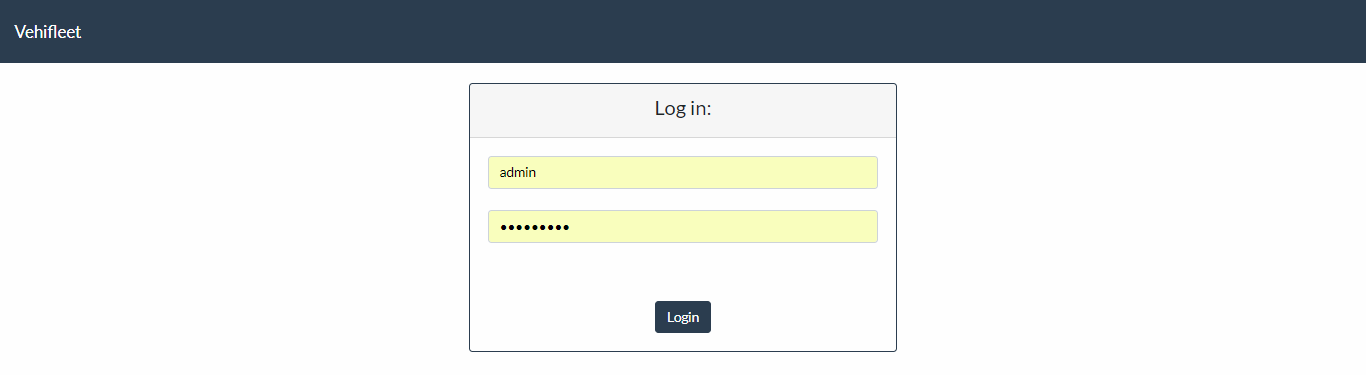
\includegraphics[width=\textwidth]{images/views/dashboard-login.png}
		\caption{Widok logowania (dashboard-login).}
		\small 
		Jedyny widok dostępny dla niezalogowanego użytkownika. Aplikacja uniemożliwia dostęp do wszystkich innych widoków osobom niezalogowanym; przy ręcznej zmianie adresu w przeglądarce nieupoważniony użytkownik zostanie przekierowany do tego widoku.
	\end{figure}
	
	%\subsection{Ekran wylogowywania}
	\begin{figure}[H]
		\centering
		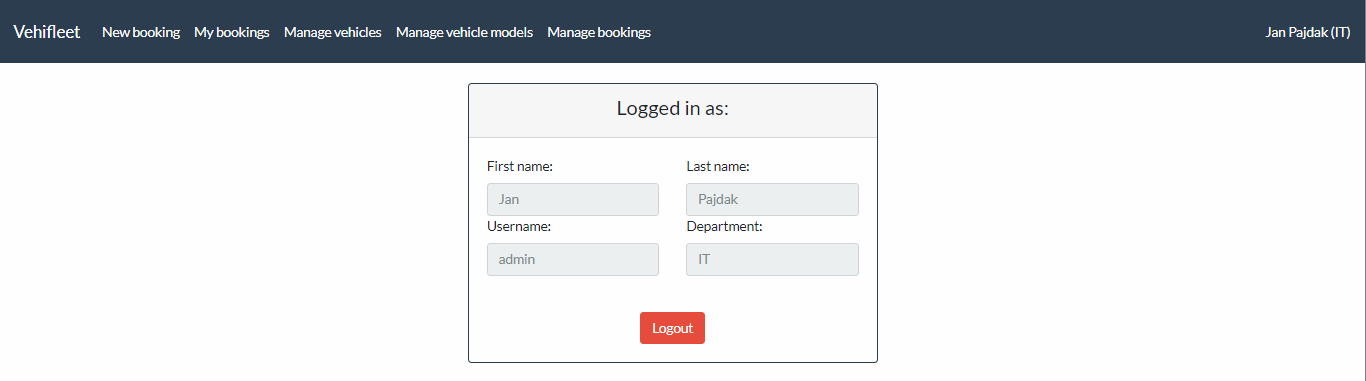
\includegraphics[width=\textwidth]{images/views/dashboard-logout.png}
		\caption{Widok zalogowanego użytkownika (dashboard-user-details).}
		\small 
		Podstawowy widok zalogowanego użytkownika z informacjami o użytkowniku i możliwością wylogowania się.
	\end{figure}
	
	%\subsection{Dostępne pojazdy}
	\begin{figure}[H]
		\centering
		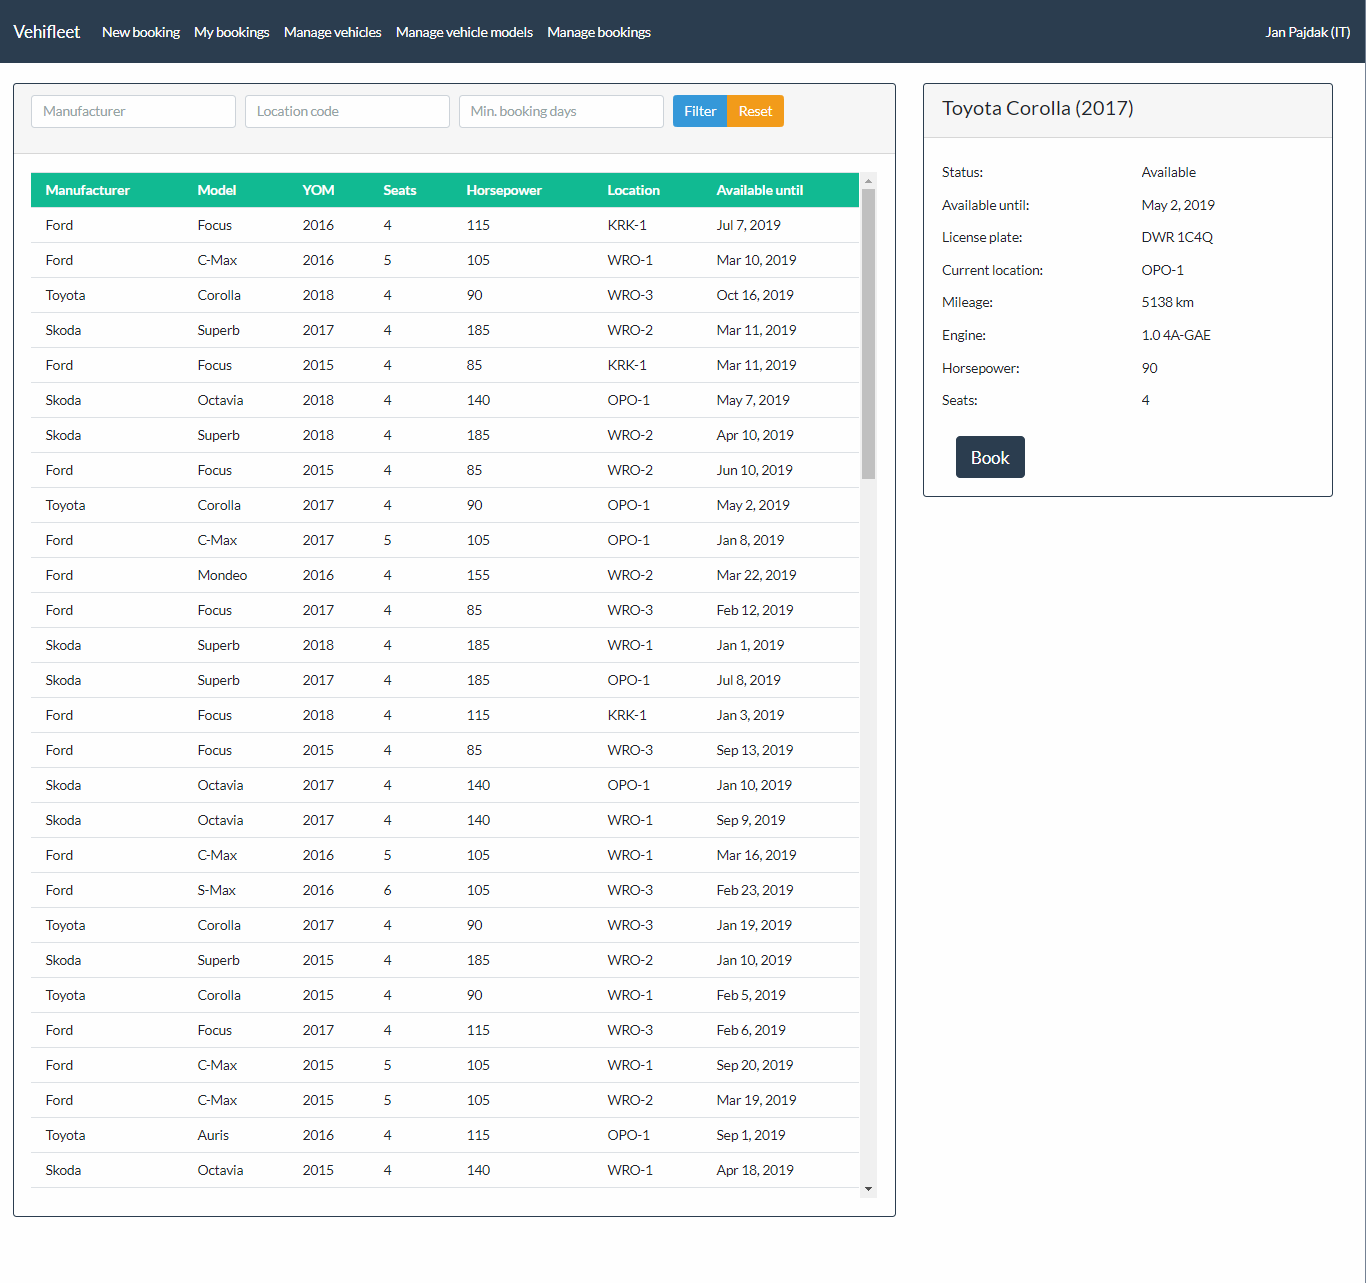
\includegraphics[width=\textwidth]{images/views/vehicle-booking-2.png}
		\caption{Widok listy dostępnych pojazdów (vehicle-list-booking).}
		\small 
		Lista dostępnych pojazdów która może być dodatkowo filtrowana. Po kliknięciu na jakikolwiek pojazd, jego dokładne informacje zostają wczytane i wyświetlone w oknie po prawej stronie; użytkownik może utworzyć nową rezerwację używając przycisku \textit{Book}.
	\end{figure}
	
	%\subsection{Historia rezerwacji}
	\begin{figure}[H]
		\centering
		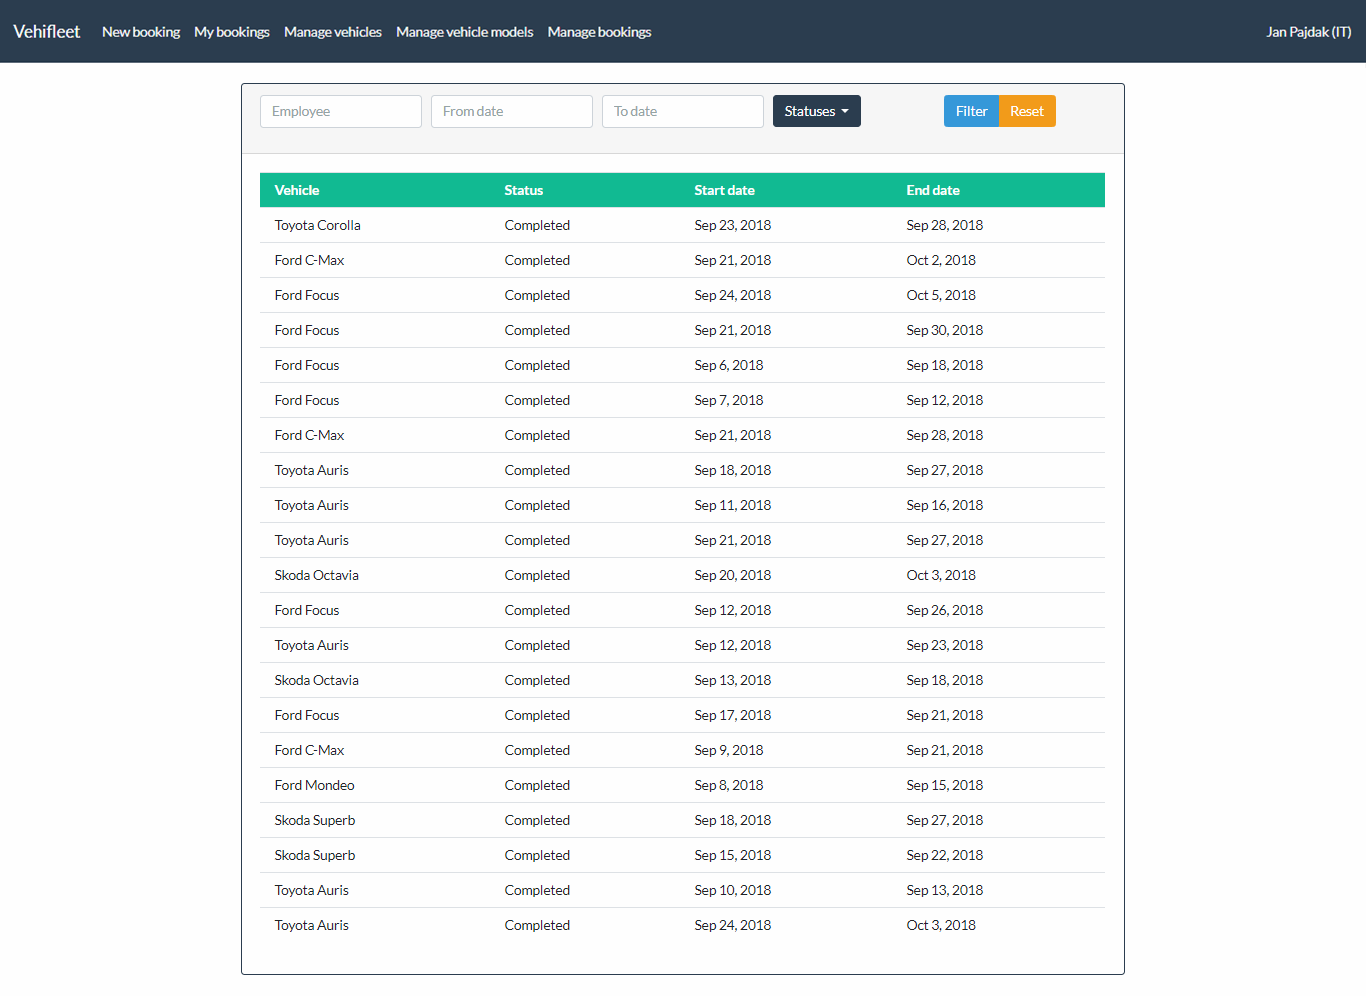
\includegraphics[width=\textwidth]{images/views/booking-list-manage.png}
		\caption{Widok listy historii rezerwacji (booking-personal).}
		\small 
		Widok zawiera rezerwacji utworzone tylko i wyłącznie przez zalogowanego użytkownika; użytkownik bez praw kierownika nie jest w stanie przeglądać cudzych rezerwacji. Kliknięcie w rekord otwiera szczegółowy widok rezerwacji.
	\end{figure}
	
	%\subsection{Szczegóły rezerwacji}
	\begin{figure}[H]
		\centering
		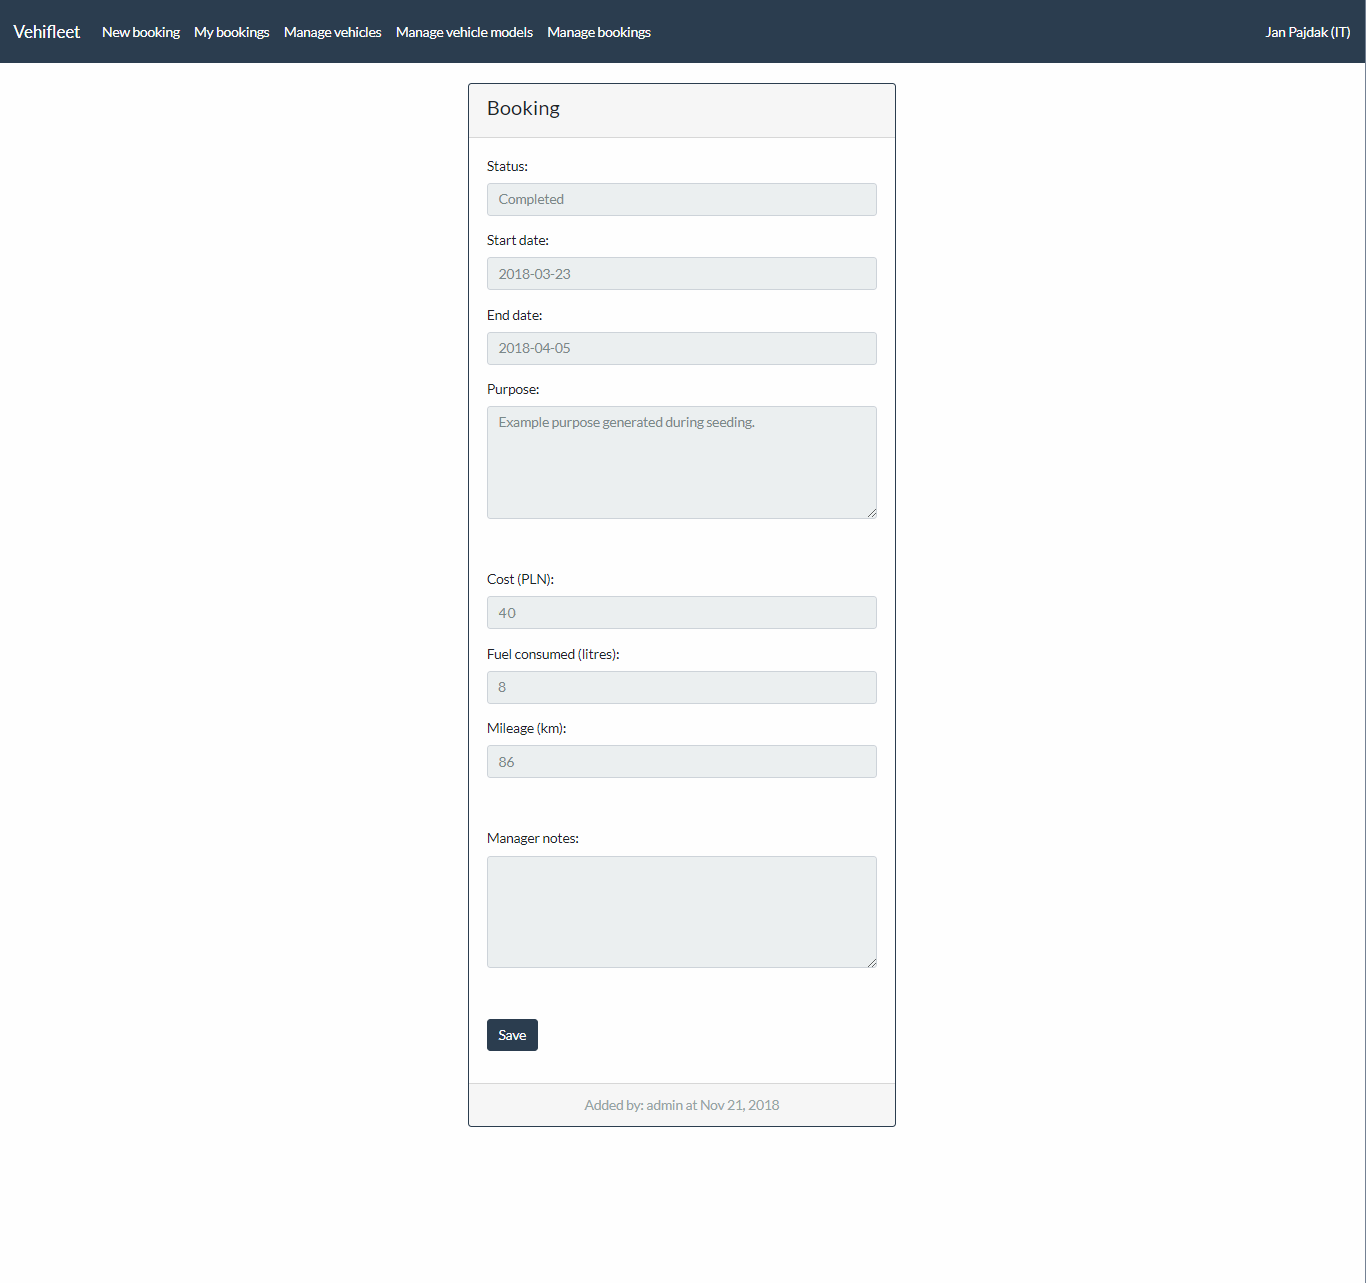
\includegraphics[width=\textwidth]{images/views/booking-detail.png}
		\caption{Widok szczegółowy rezerwacji (booking-details).}
		\small 
		W tym widoku można zarówno utworzyć nowe rezerwację, jak i edytować już istniejące.
	\end{figure}
	
	%\subsection{Szczegóły rezerwacji w trybie kierownika}
	\begin{figure}[H]
		\centering
		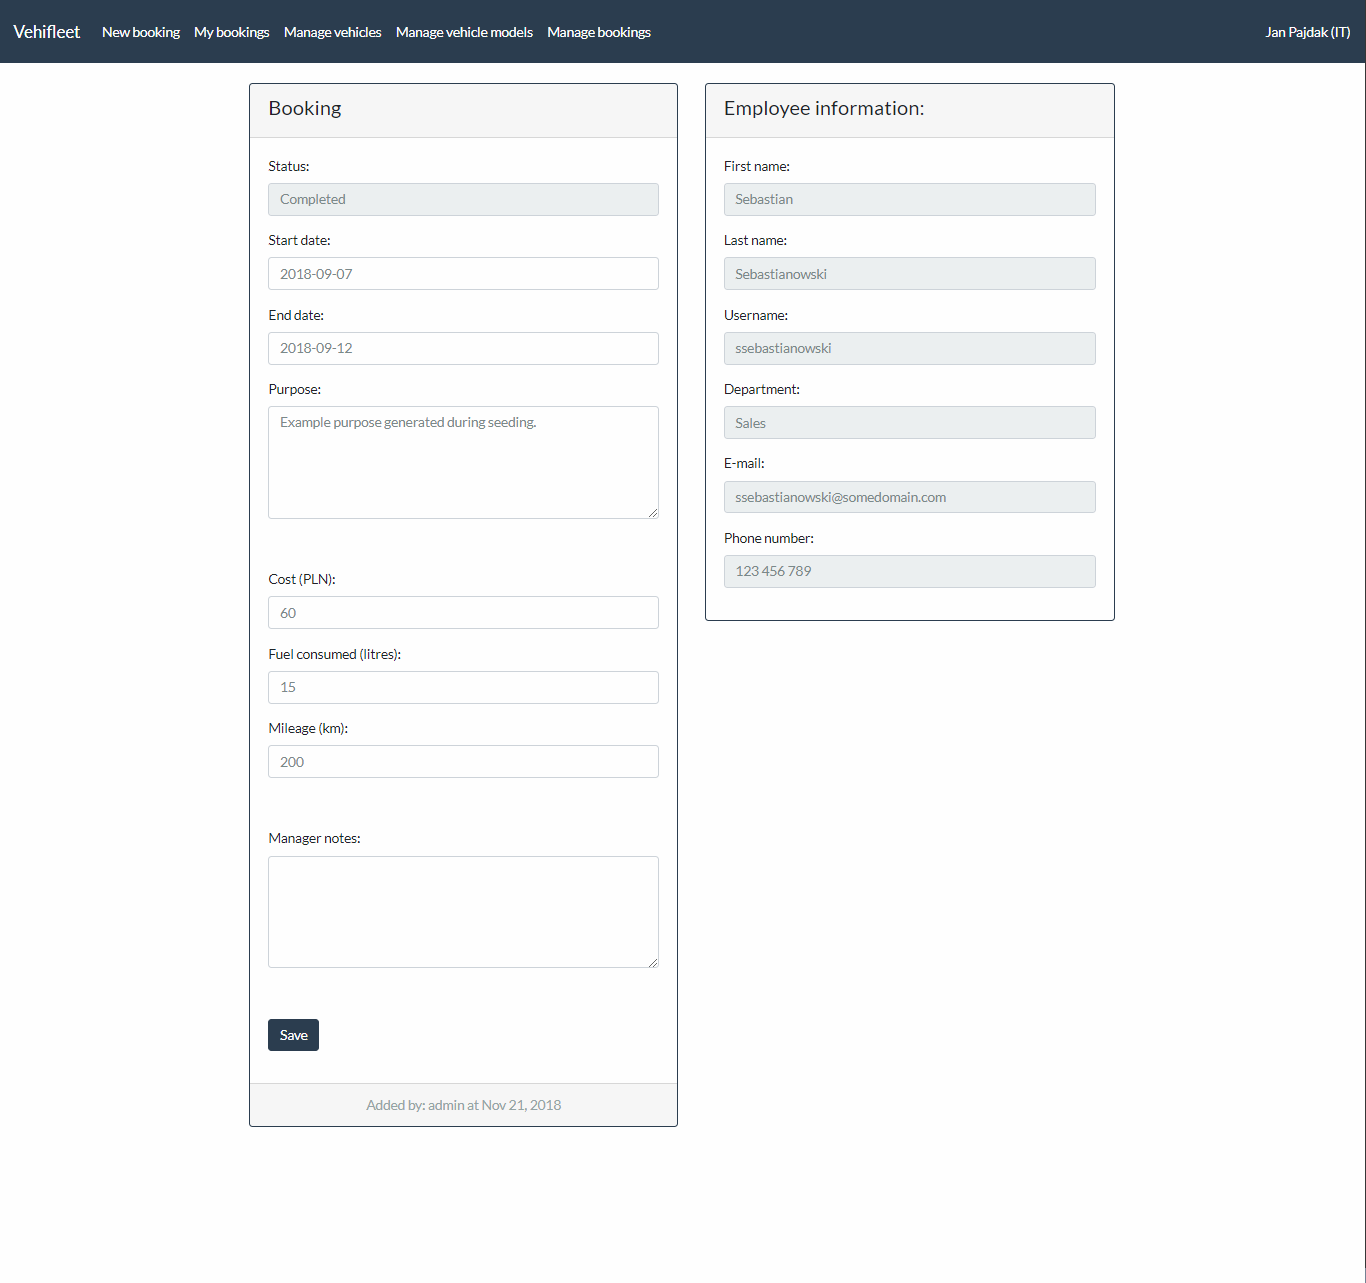
\includegraphics[width=\textwidth]{images/views/booking-detail-manager.png}
		\caption{Widok szczegółowy rezerwacji w trybie kierownika (booking-details).}
		\small 
		Jeżeli zalogowany użytkownik posiada pełne uprawnienia i przegląda cudze rezerwacji, po stronie prawej zostają wyświetlone dodatkowe informacje o użytkowniku który utworzył rezerwację.
	\end{figure}
	
	%\subsection{Wszystkie pojazdy}
	\begin{figure}[H]
		\centering
		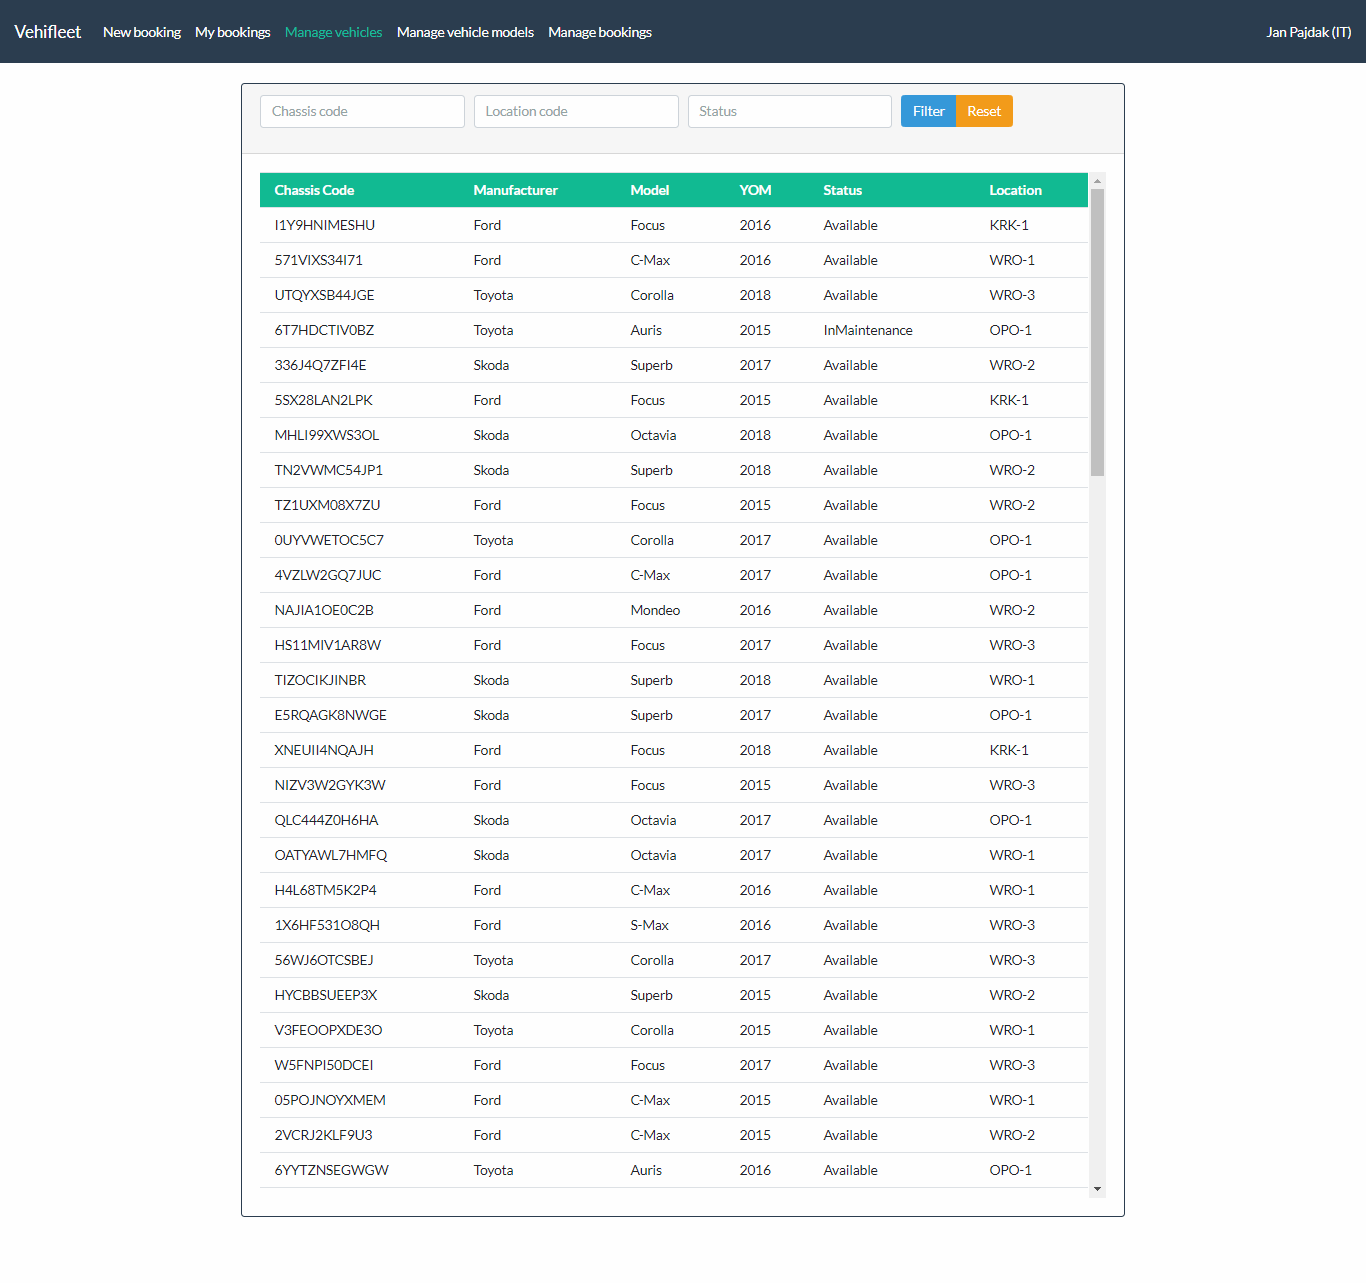
\includegraphics[width=\textwidth]{images/views/vehicle-list.png}
		\caption{Widok listy pojazdów (vehicle-list).}
		\small 
		Widok pozwala na przeglądanie wszystkich pojazdów śledzonych w systemie oraz na filtrowanie. Kliknięcie w rekord przechodzi do widoku szczegółów wybranego pojazdu.
	\end{figure}
	
	%\subsection{Szczegóły pojazdu}
	\begin{figure}[H]
		\centering
		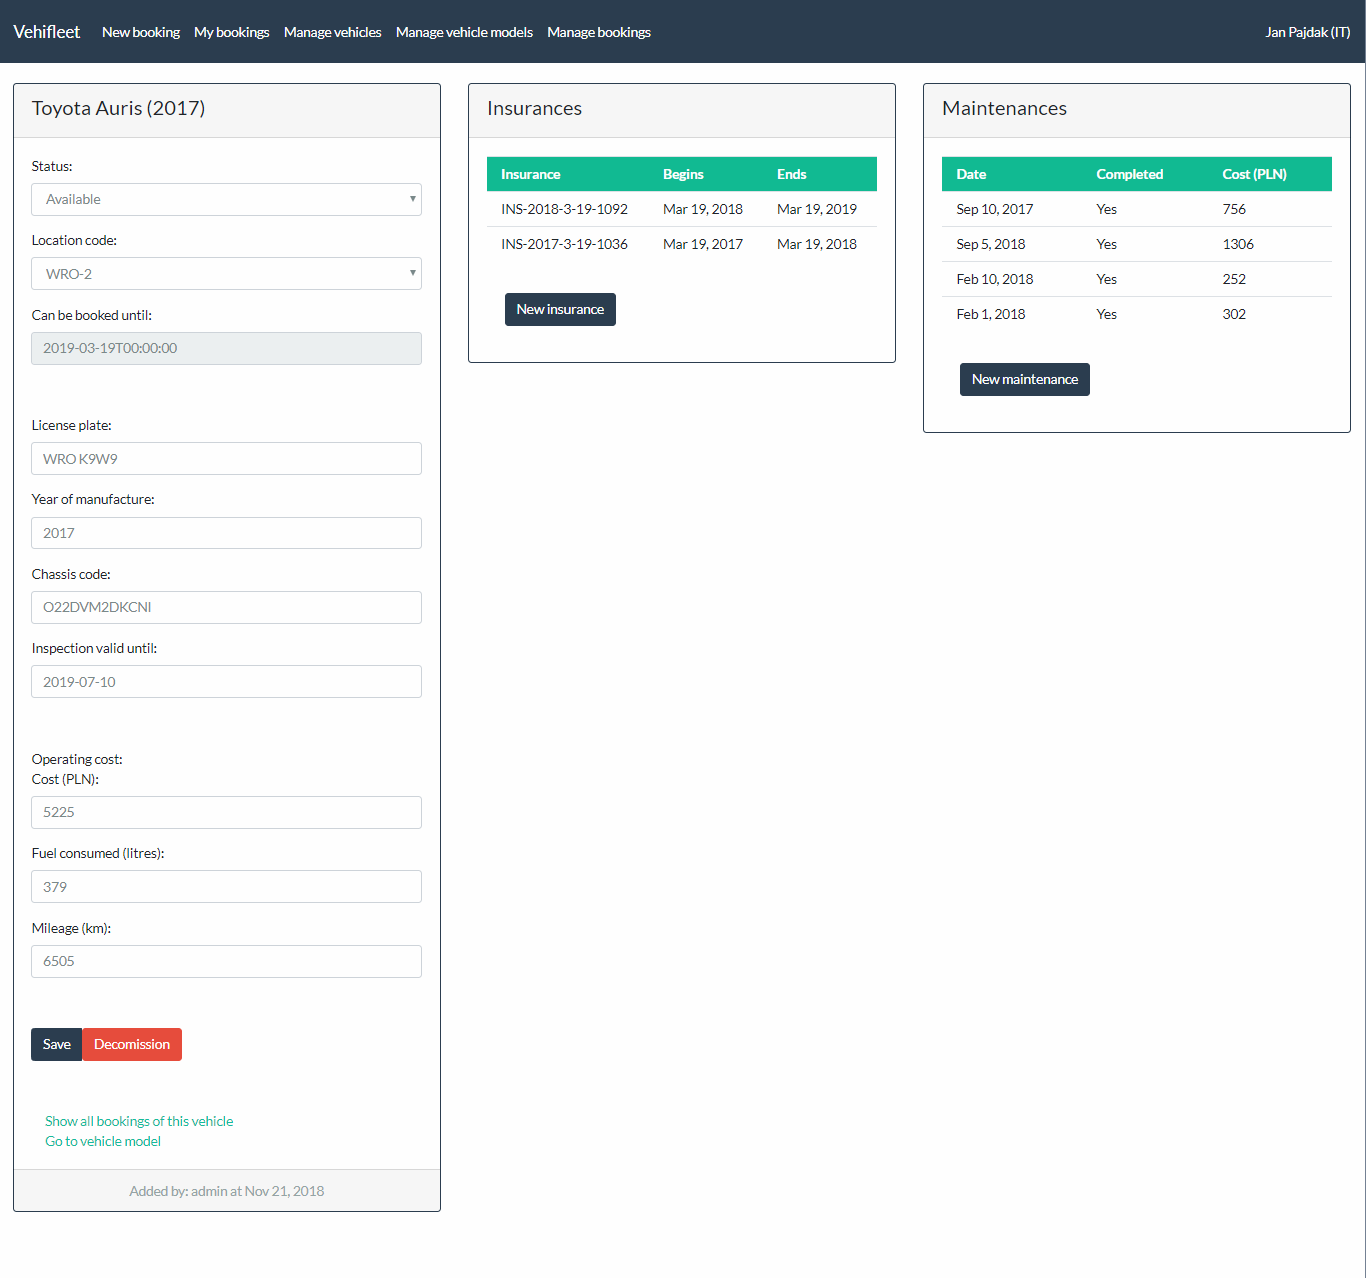
\includegraphics[width=\textwidth]{images/views/vehicle-detail.png}
		\caption{Widok szczegółowy pojazdu (vehicle-details).}
		\small 
		Widok zawierający wszystkie informacje na temat pojazdu wraz z listą ubezpieczeń i napraw, które mogą być dodawane lub edytowane po wybraniu poprzez kliknięcie. Użytkownik może wyświetlić wszystkie rezerwacji danego pojazdu lub jego dokładną specyfikacje techniczną po kliknięciu na jeden z dwóch odnośników na dole okna.
	\end{figure}
	
	%\subsection{Szczegóły ubezpieczenia}
	\begin{figure}[H]
		\centering
		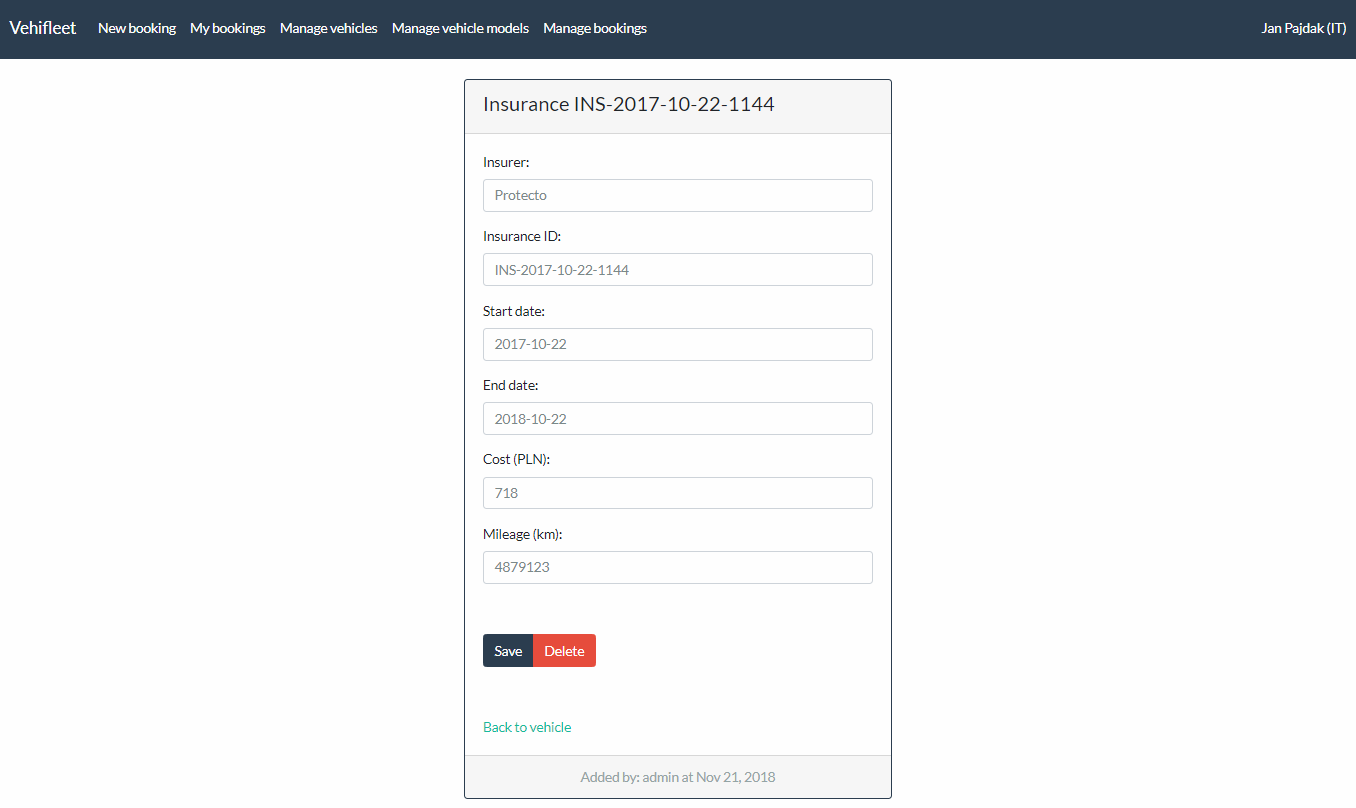
\includegraphics[width=\textwidth]{images/views/insurance-detail.png}
		\caption{Widok szczegółowy ubezpieczenia (insurance-details).}
		\small 
		Widok pozwalający na edycję ubezpieczenia.
	\end{figure}
	
	%\subsection{Szczegóły naprawy}
	\begin{figure}[H]
		\centering
		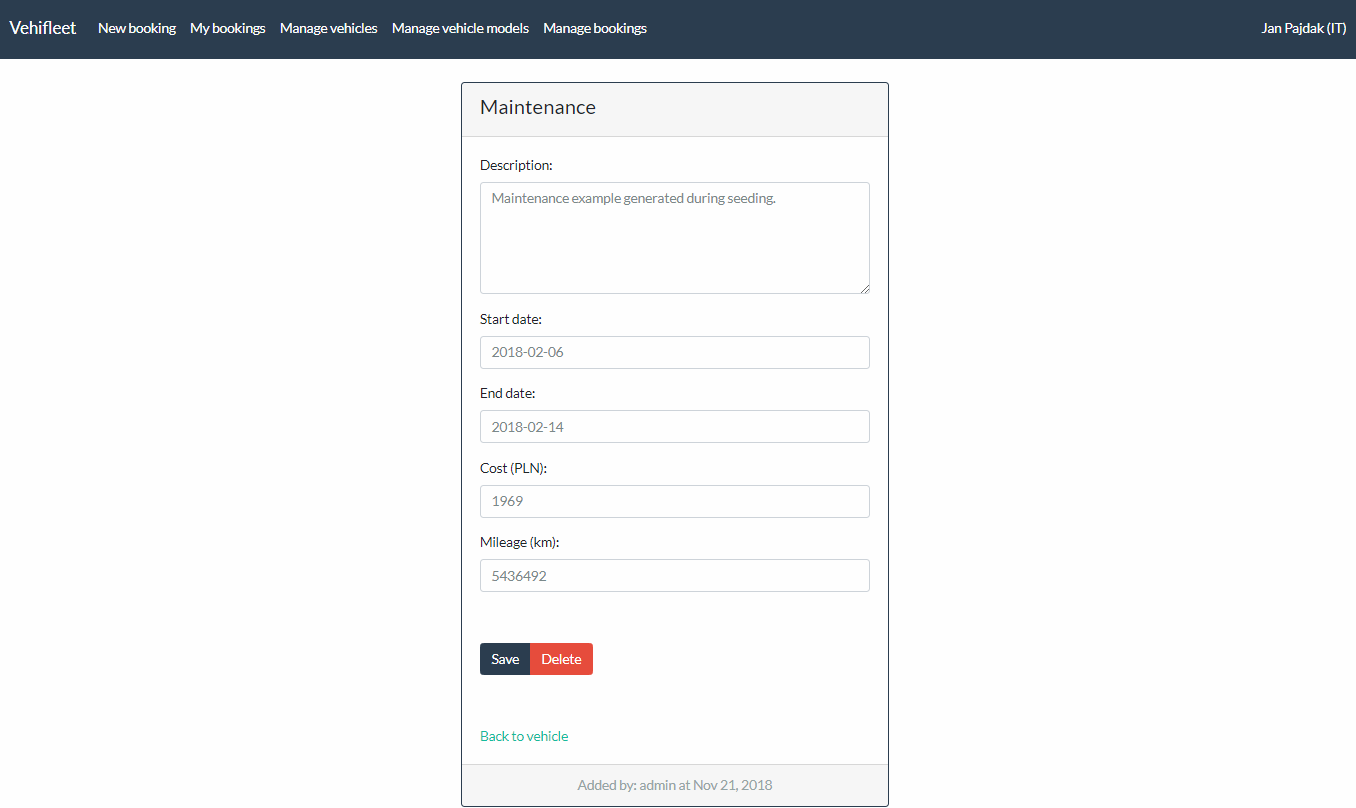
\includegraphics[width=\textwidth]{images/views/maintenance-detail.png}
		\caption{Widok szczegółowy naprawy (maintenance-details).}
		\small 
		Widok pozwalający na edycję zdarzenia naprawy.
	\end{figure}
	
	%\subsection{Wszystkie modele pojazdów}
	\begin{figure}[H]
		\centering
		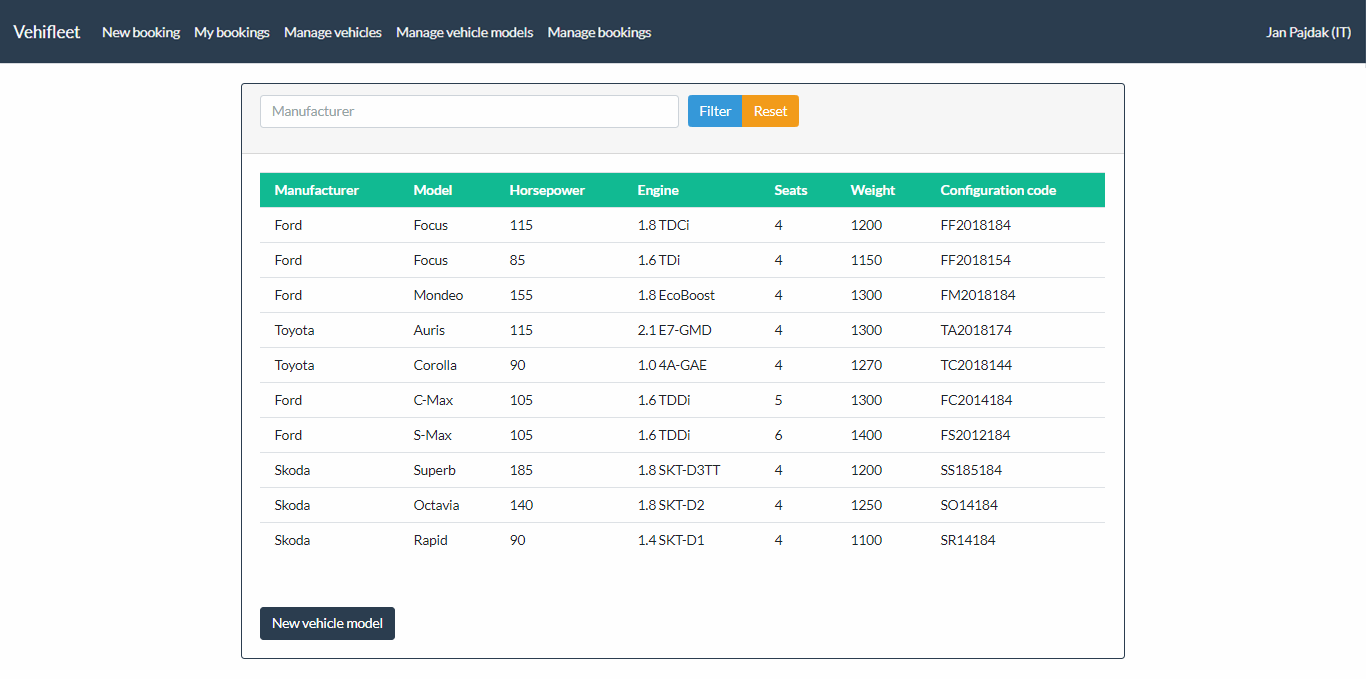
\includegraphics[width=\textwidth]{images/views/vehicle-model-list.png}
		\caption{Widok listy modeli pojazdów (vehicle-model-list).}
		\small 
		Widok umożliwia przeglądanie modeli pojazdów. Kliknięcie w rekord przechodzi do widoku szczegółowego. 
	\end{figure}
	
	%\subsection{Szczegóły modelu pojazdu}
	\begin{figure}[H]
		\centering
		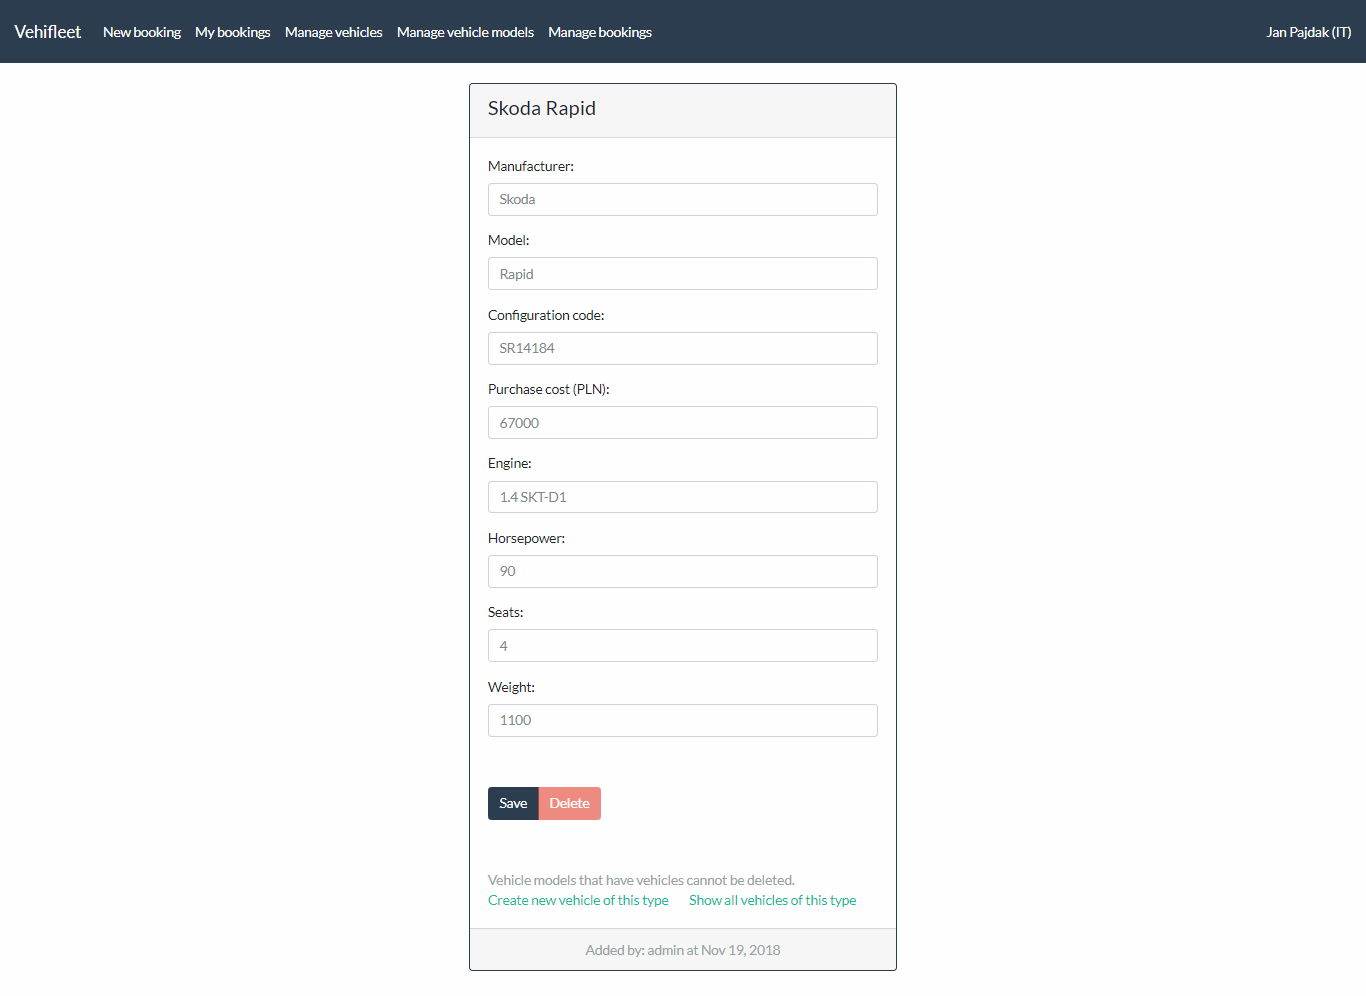
\includegraphics[width=\textwidth]{images/views/vehicle-model-detail.png}
		\caption{Widok szczegółowy modelu pojazdu (vehicle-model-details).}
		\small 
		Widok pozwalający na dodawanie oraz edycje modeli pojazdów. Użytkownik może również wyświetlić wszystkie pojazdy tego typu lub wprowadzić informację o nowym egzemplarzu za pomocą odnośników na dole okna.
	\end{figure}
	%----------------------------------------------------------------------------------------
	%	SECTION OLD
	%----------------------------------------------------------------------------------------
	
	%\chapter{Projekt systemu}
	%System można podzielić na dwa elementy — interfejs użytkownika (\textit{UI}) oraz interfejs programistyczny (\textit{API}). Komunikacja między interfejsami odbywa się według protokołu \textit{HTTP}; dane przesyłane są w formacie \textit{JSON}.
	%
	%Dostęp do systemu został zabezpieczony przy użyciu standardu \textit{JSON Web Token (JWT)}. Autoryzacja \textit{JWT} działa w następujący sposób:
	%\begin{enumerate}
	%	\item Użytkownik loguje się przez interfejs użytkownika, podając nazwę użytkownika oraz hasło
	%	\item Interfejs programistyczny weryfikuje dane logowania
	%	\item W przypadku prawidłowego hasła utworzony zostaje token \textit{JWT} zawierający:
	%		\subitem Informacje o wydającym token
	%		\subitem Informacje o użytkowniku: jego identyfikator (nazwa użytkownika) oraz role
	%	\item Utworzony token zostaje zaszyfrowany (uniemożliwiając jego sfałszowanie)i przesłany 		
	%	\item Odebrany token zostaje umieszczony w pamięci przeglądarki internetowej użytkownika
	%\end{enumerate}
	%Interfejs programistyczny weryfikuje poprawność tokena dla każdego żądania \textit{HTTP} z wyjątkiem tych związanych z procesem autoryzacji użytkownika; jeżeli token jest niepoprawny lub zbyt stary (wydany więcej niż 2 godziny przed weryfikacją), żądanie jest odrzucone.
	%
	%
	%[[ tutaj dodam zdjęcie tokenu z systemu przed i po szyfrowaniu ]]
	
	%----------------------------------------------------------------------------------------
	%	APPENDIX
	%----------------------------------------------------------------------------------------
	%\appendix
	%\chapter{Donec cursus nulla vitae pede}
	%Donec cursus nulla vitae pede. Etiam quam pede, aliquet ut, pellentesque sed, sagittis non, est. Quisque egestas malesuada risus. Maecenas ultricies libero a quam. Nullam feugiat arcu. Class aptent taciti sociosqu ad litora torquent per conubia nostra, per inceptos hymenaeos. In interdum, risus ut gravida sollicitudin, leo sapien commodo dui, non consectetuer nisl nunc ac massa. Mauris a orci in eros venenatis euismod. Curabitur orci. Quisque pharetra, dui sed dignissim hendrerit, nibh ante malesuada eros, sed tincidunt magna lorem a tellus. Aliquam erat volutpat. Aenean pulvinar, metus et mattis dictum, massa lacus semper purus, quis vehicula augue mi et leo. Ut eu ipsum. Sed dictum dapibus nisi. Cras mattis.
	
	%----------------------------------------------------------------------------------------
	%	END
	%----------------------------------------------------------------------------------------
	\addcontentsline{toc}{chapter}{Literatura}
	\bibliography{bibliography}
	
	%opcjonalnie może się tu pojawić spis rysunków i tabel
	\newpage
	\listoffigures
	\newpage
	\listoftables
	\newpage
	\lstlistoflistings
\end{document}

